\documentclass{article}
\usepackage[utf8]{inputenc}
\usepackage{amsmath, amsthm, amssymb, mathpazo, isomath, mathtools}
\usepackage{subcaption,graphicx}
\usepackage{fullpage}
\usepackage{booktabs}
\usepackage{hyperref}
\usepackage{algorithm, algorithmic}
\usepackage{mathtools}
\usepackage{todonotes}

\newcommand{\example}[1]{\todo[inline,color=green!30!white]{\textbf{Example:} #1}}

\title{Notes for Numerical Analysis of PDEs and related topics}
%\author{Nicol\'as A Barnafi\thanks{Instituto de Ingeniería Biológica y Médica, Pontificia Universidad Católica de Chile, Chile}, Axel Osses\thanks{Departamento de Ingeniería Matemática, Universidad de Chile, Chile}}
\author{Nicol\'as A Barnafi}
%\date{}

\renewcommand{\vec}{\vectorsym}
\newcommand{\mat}{\matrixsym}
\newcommand{\ten}{\tensorsym}
\DeclareMathOperator{\grad}{\nabla}
\DeclareMathOperator{\dive}{\text{div}}
\DeclareMathOperator{\curl}{\text{curl}}
\newtheorem{remark}{Remark}
\newtheorem{definition}{Definition}
\newtheorem{note}{Note}
\newcommand{\R}{\mathbb{R}}
\newcommand{\D}{\mathcal{D}}
\newcommand{\T}{\mathcal{T}}
\renewcommand{\P}{\mathcal{P}}

\newcommand{\tin}{\text{in }}
\newcommand{\ton}{\text{on }}

\newtheorem{theorem}{Theorem}
\newtheorem{lemma}{Lemma}

\usepackage{listings}
\usepackage{xcolor}
\definecolor{codegreen}{rgb}{0,0.6,0}
\definecolor{codegray}{rgb}{0.5,0.5,0.5}
\definecolor{codepurple}{rgb}{0.58,0,0.82}
\definecolor{backcolour}{rgb}{0.95,0.95,0.92}
\lstdefinestyle{mystyle}{
  backgroundcolor=\color{backcolour}, commentstyle=\color{codegreen},
  keywordstyle=\color{magenta},
  numberstyle=\tiny\color{codegray},
  stringstyle=\color{codepurple},
  basicstyle=\ttfamily\footnotesize,
  breakatwhitespace=false,         
%   breaklines=false,                     
  captionpos=b,                    
  keepspaces=true,                 
  numbers=none,                    
  numbersep=5pt,                  
  showspaces=false,                
  showstringspaces=false,
  showtabs=false,                  
  tabsize=2,
%   frameround=tttn,
  framerule=1.5pt,
  rulecolor=\color{red!60!black}
}
\lstset{style=mystyle}

\begin{document}

\maketitle

\section*{Context}

These notes exist as backup material for a course on some deeper topics in Math Eng at Pontificia Universidad Católica de Chile, the 2nd semester of 2024. The idea is to provide mathematical tools for students that give them the ability to assess the difficulty of mathematical problems, mainly within the world of Partial Differential Equations (PDEs). The target is ultimately to implement these models, so that all tools are oriented towards having solid foundations that allows one to trust a computational model. Informally speaking, the main mathematical concepts to haunt us during all these notes are: 
    \begin{itemize}
        \item Existence and uniqueness: It is a natural baseline in the mathematician's world to try to solve only problems that \emph{have} a solution. Otherwise, things might be as pointless as developing an iterative method for finding real numbers such that $x^2 = -1$. Uniqueness is a further luxury, but sometimes two different methods give two different solutions, and having only those things at hand can make it difficult to distinguish whether that is a bug or a feature of the model. There exist some root-isolation methods that allow to find solutions of a problem that are \emph{different} from a given one. This is out of the scope of this course. 
        \item Stability: The intuitive idea behind this is that small perturbations in the data give rise to small changes in the solution. This typically looks like 
            $$ \| u\|_X \leq \| f\|_{X'}, $$
        where $u$ is the solution of a problem that depends on $f$, and $X$ is some functional (hopefully Hilbert) space. More rigorously, this means that the solution map $f \mapsto u(f)$ is bounded, or continuous in the linear case. Stability also sometimes refers to time dynamics and the fact that a discrete solution stays \emph{within a certain distance} of the real solution throughout a simulation. In the continuous setting, it might also mean that there are no finite-time singularities. In general, stability is not a well defined term, but still a widely understood one to anyone who has struggled to get a code to run correctly, and a highly desired property. 
    \end{itemize}
All other properties (or at least most of them anyway) are ways to guarantee that a problem enjoys one of these nice properties. There are ways to handle problems that do not have those properties, but they are almost always extremely problem dependent, and the person studying such problems should dive deep into the sectorial knowledge to see how certain communities deal with such issues. This is an aspect that mathematically oriented people almost always disregard, which has some severe mathematical (and social) consequences. In fact, some extremely classical models in engineering are still far from understood mathematically, such as the Navier-Stokes equations. This has not prevented the CFD community from solving these models with extreme efficiency, and from further leveraging them for industrial applications which, unsurprisingly, work fantastically. Discovering the amazing ways in which mathematically obvlivious communities solve mathematically hard problems is, and will probably be for very long, a beautiful opportunity for collaboration.

%%%%%%%%%%%%%%%%%%%%%%%%%%%%%%%%%%%%%%%%%%%%%%%%%%%%
%%%%%%%%%%%%%%%%%%%%%%%%%%%%%%%%%%%%%%%%%%%%%%%%%%%%
\section{Finite differences}
This section has been heavily extracted from some notes from the WIAS in Berlin. They didn't have any authorship, so I don't really know who to thank for them.  Probably the simplest (and oldest) idea for approximating equations stems from the use of Taylor's theorem:

\begin{theorem}\label{thm:taylor}
    Consider a function $f$ in $C^n((a,b), \R)$, i.e. $n$ times differentiable whose derivatives are well-defined in $a$. Then, there is some $\xi$ in $(a,b)$ such that
    $$ f(b) = \sum_{k=0}^{n-1}\frac{f^{(k)}(a)}{k!}(b-a)^k + \frac{f^{(n)}(\xi)}{n!}(b-a)^n. $$
\end{theorem}
Naturally, this is the mean value theorem when $n=1$. From now on we consider our setting to be in $\R$. For any continuous function $f:(a,b)\to \R$, we can define its associated \emph{grid function} given by its evaluation in a finite set of points. We sometimes refer to this as \emph{collocation}. Set $a<b$, and define the points $a=x_1<\hdots<x_N=b$ with $h_i=x_{i}-x_{i-1}$, such that we have $N$ points, and define the grid function as the vector
    $$ R_hf = (f_1, \hdots, f_N) \coloneqq (f(x_1), \hdots, f(x_N)) \in \R^N,$$
    where we have defined the $R_h$ operator such that $R_hf:\R^N \to \R^N$ and $R_h:C((a,b),\R)\to [\R^N\to\R^N]$.  We can then define the following difference operators: 
    \begin{itemize}
        \item Forward difference: 
            $$ D^+f(x_i) \coloneqq \frac{f_{i+1} - f_i}{h_{i+1}} $$
        \item Backward difference: 
            $$ D^-f(x_i) \coloneqq \frac{f_{i} - f_{i-1}}{h_{i}} $$
        \item Centered difference:
            $$ Df(x_i) \coloneqq \frac{f_{i+1} - f_{i-1}}{h_{i+1} - h_{i-1}} $$

    \end{itemize}
A nice simple excercise is to extend these ideas to second order derivatives, which all stem from Taylor's formula. The application we will be interested is in that of approximating the action of a differential operator using these formulas. For this, we will focus on the forward difference formula. At each grid point we will have
$$ D^+f(x_i) = \frac{f_{i+1} - f_i}{h_{i+1}} = \frac 1{h_{i+1}} [-1\quad 1]\begin{bmatrix}f_i \\ f_{i+1}\end{bmatrix}, $$
so that defining the matrix $\mat D_h^+$ in $\R^{N\times N}$ as
$$ [\mat D_h^+]_{ij} = \begin{cases} -1/h_{i+1} & j=i \\ 1/h_i  & j=i+1 \\ 0 & \text{elsewhere} \end{cases} $$
we obtain an operator which, given a grid function, it yields its discrete derivative. Naturally, care has to be taken at the last point, where we can simply use instead a backwards difference. 

Finite difference approximations can be easily seen to be convergent for sufficiently smooth functions. To see this, consider Taylor's theorem to obtain for $h>0$:
    $$ f(x+ h) = f(x) + f'(x)h + O(h^2), $$
from which we readily obtain that 
    $$ | D^+f(x) - f'(x) | = O(h), $$
    so that forward differences and also backward differences (straightforward calculation) converge pointwise linearly. 

\begin{figure}
    \centering
    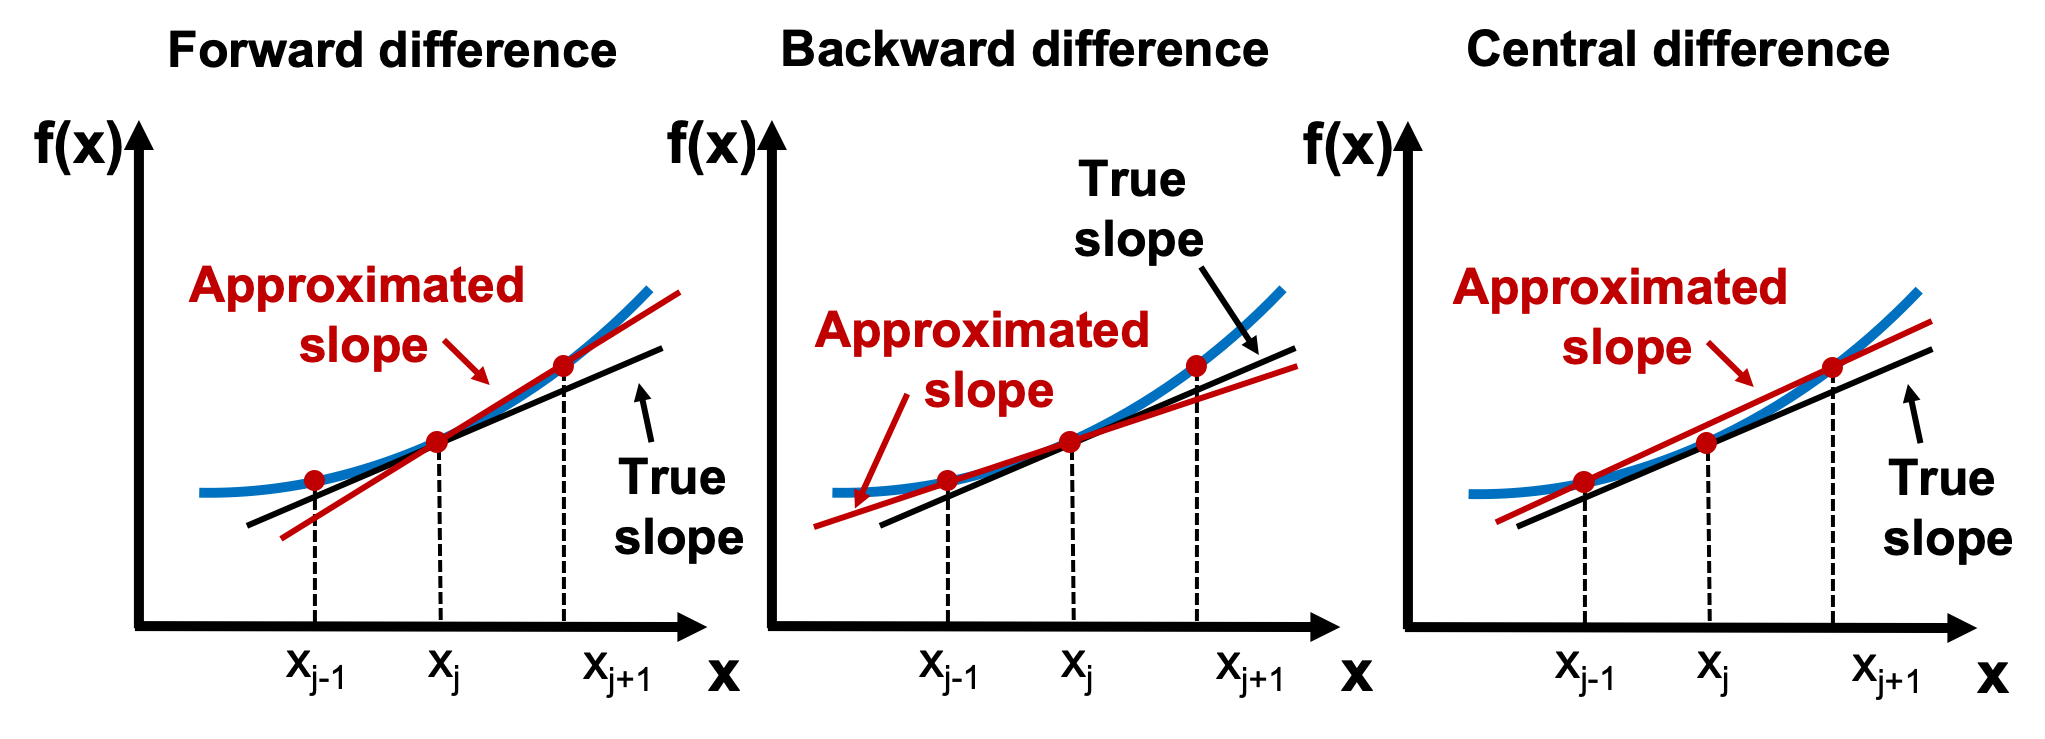
\includegraphics[width=\linewidth]{figuras/fdm_convergence.png}
    \caption{Forward, centered and backward difference schemes for calculating the first derivative. Retrieved from \href{https://pythonnumericalmethods.studentorg.berkeley.edu/notebooks/chapter20.02-Finite-Difference-Approximating-Derivatives.html}{this website}, which shows a simple implementation of the forward scheme using NumPy.}
\end{figure}

\subsection{Second order derivatives}
The standard way of approximating second order derivatives is that of using a finite difference approximation twice. It is given by the following: 
$$ \begin{aligned}
    f''(x) &\approx D^+(f')(x) \\
           &=\frac{f'(x+h) - f'(x)}{h} \\
           &\approx\frac{\frac{f(x+h) - f(x)}{h} - \frac{f(x) - f(x-h)}{h}}{h} \\
           &= \frac{f(x+h) - 2f(x) + f(x-h)}{h^2}.
    \end{aligned}
$$
We note that the intermediate steps show that these computations can be represented as the matrix product $\mat D^+ \mat D^-$, where the order of differentiation can be inverted and thus equivalently $\mat D^- \mat D^+$. 
\subsection{Order of convergence}
The order of convergence of the previously computed schemes can be derived from Taylor's theorem. For example, we previously showed that backward/forward differences converge linearly (pointwise), and indeed we can do the same for centered differences. For this, consider the following third order expansions:
    $$
    \begin{aligned}
        f(x+h) &= f(x) + hf'(x) + \frac {h^2} 2 f''(x) + \mathcal O(h^3) \\
        f(x-h) &= f(x) - hf'(x) + \frac {h^2} 2 f''(x) + \mathcal O(h^3),
    \end{aligned}
    $$
and by simply adding both equations it can be shown that the finite difference formula computed converges linearly.


\subsection{Convergence Analysis}
Using these ideas, we can now proceed to propose a mechanisms for discretizing differential operators. A central question regards the capability of approximation that such an objects has, which finds its answer in Lax's theorem. We will first require other definitions. 

\begin{definition}[Consistency]
    Consider some differential operator $\mathcal A$. A discrete operator $\mat A_h$ in $\R^{N\times N}$ is said to be \emph{consistent} with $\mathcal A$ of order $k$ if for all sufficiently smooth functions it holds that
    $$ \max_{i\in\{1,\hdots,N\}}|\mathcal Af(x_i) - [\mat A_hR_hf]_i| =: \|R_h \mathcal Af - \mat A_hR_h f\|_{\infty,h} \leq C h^k, $$
    where $\|\cdot \|_{\infty,h}$ is the induced infinity norm in $\R^N$ and $C$ is a positive constant independent of $h$. This is sometimes stated more weakly by saying that the norm is $\mathcal O(h^k)$. 
\end{definition}

\example{The difference operators are all consistent with the first order derivative, which can be seen immediately from Taylor's theorem.}
\begin{definition}[Stability]
    A finite difference operator $\mat A_h$ is said to be stable (in the discrete maximum norm) if there is a stability constant $C>0$ that does not depend on the grid size such that
        $$ \| \vec v_h \|_{\infty,h} \leq C \|\mat A_h \vec v_h \|_{\infty,h}$$
        for all grid functions $\vec v_h$. 
\end{definition}
We finally consider an infinite dimensional problem given by
    $$ \mathcal A u = f $$
and its finite difference approximation as
    $$ \mat A_h \vec u_h = \vec f_h, $$
    which will allow us to define convergence. 

\begin{definition}[Convergence]
    The finite differences scheme is said to be convergent of order $k$ in the discrete maximum norm if the discrete solution and the continuous one satisfy that 
    $$ \| \vec u_h - R_hu \|_{\infty,h} \leq C h^k. $$
This is sometimes stated more weakly by saying simply that $\| \vec u_h - R_hu \|_{\infty,h}$ is $\mathcal O(h^k)$. 
\end{definition}

\begin{theorem}
    Consider the previously defined problem and its finite difference discretization. If the scheme is consistent, then stability and convergence are equivalent. 
    \begin{proof}
        The stability to convergence part is taken directly from the aforementionted notes. The convergence to stability is instead partly inspired by the notes by Long Chen on abstract convergence analysis \cite{chenLFDM}.
        
        {\bf Step 1, Stability implies convergence:}

        We proceed directly through inequalities:
        \begin{align*}
            \| \vec u_h - R_h u\|_{\infty,h} &\leq C\|\mat A_h(\vec u_h - R_hu) \|_{\infty,h} && \text{(Stability)} \\
                                             &=C \| f_h - \mat A_hR_h u \|_{\infty,h} && \\
                                             &=C \| R_h f - \mat A_hR_h u\|_{\infty,h} &&\\
                                             &=C \|R_h(\mathcal A u) - \mat A_hR_h u\|_{\infty,h}&& \\
                                             &\leq Ch^k && \text{(Consistency)}.
        \end{align*}

        {\bf Step 2, Convergence implies stability:}

        We note that stability can be read, by taking inverses, as 
        $$ \| \mat A_h^{-1}\vec f_h \|_{\infty, h} \leq C \|\vec f_h\|_{\infty, h}. $$
        which is simply the continuity of the inverse map $\mat A_h^{-1}$. Consider an arbitrary grid vector $\vec f_h$, and we denote the associated problem solution as $\vec u_h$, where $\mat A_h \vec u_h = \vec f_h$. Using this, we have that
        $$ 
        \begin{aligned} 
            \|\mat A_h^{-1}\vec f_h\|_{\infty,h} &= \| \vec u_h \|_{\infty, h} \leq \| \vec u_h - R_h u \|_{\infty, h} + \| R_h u \|_{\infty, h} && \text{(Convergence)}\\
                                                 &\leq C h^k + \| R_h \mathcal A^{-1} f \|_{\infty, h}. 
        \end{aligned}
        $$
        To bound this last term, we note that $R_h$ yields pointwise evaluations, so for any continuous function $\eta$ it will hold that
        $$ \| R_h \eta \|_{\infty,h} \leq \| \eta \|_0, $$
        where $\| \eta \|_0$ is the supremum norm. Finally, we use that $\mathcal A$ is a continuous bijection, and thus from the open mapping theorem it holds that $\|\mathcal A^{-1}\|$ is bounded by some constant $C_2$. Using this fact, the previous estimate becomes 
        $$ \| \mat A_h^{-1} \vec f_h \|_{\infty,h} \leq Ch^k + \| \mathcal A f \|_0 \leq C h^k + C_2 \| \vec f_h \|_0<\infty, $$
        which in particular shows that $ \| \mat A_h^{-1} \vec f_h \|$ is bounded for all $\vec f_h$. The uniform boundedness principle them yields that $\mat A_h^{-1}$ is bounded, which concludes the proof.
    \end{proof}
\end{theorem}
\subsection{The empirical convergence rate}
One issue that is always overviewed is the computation of the \emph{observed} convergence rate, so we will write it here once and for all so that it is never an issue again. Assume that some error $\vec e_h$ converges to zero in some $X$ norm with rate $k$:
    $$ \|\vec e_h\|_X \leq C h^k.$$
    Then, given a sequence of mesh sizes $h$ and errors as $(h_j, [\vec e_h]_j)$, we would like to estimate $k$ to validate we really obtained the computed rate $k$. For this, we take the logarithm of the error expression:
    $$ \log \|[\vec e_h]_j\|_X \leq \log C + k \log h_j, $$
and note that we obtain roughly a line equation if we assume an equality. Because of this, we can estimate now estimate the slope of our line equation using two consecutive points as
$$ k \approx \frac{\log \|[\vec e_h]_{j+1}\|_X - \log \|[\vec e_h]_j\|_X}{ \log h_{j+1} - \log h_j}, $$
which yields the classical expression one gets everywhere: 
    $$ k \approx  \frac{\log \left(\|[\vec e_h]_{j+1}\|_X / \|[\vec e_h]_j\|_X\right)}{ \log \left(h_{j+1} / h_j\right)}. $$

\subsection{Further discretizations}
In this section we hint on how to address numerically higher dimensional problems, and also how to include time. The stability of such schemes will be studied further ahead with the von Neumann stability analysis. 
\subsubsection{Discretization in 2D and 3D}
In typical 1D examples, one has a domain $(a,b)$ and an associated grid given by some points $\{x_i\}_i^N$ such that each index $i$ corresponds to an order of the domain, and thus naturally a finite difference operator is going to involve something like $i$ and its neighbors. This scenario would be different if, for example, one had a random ordering of the grid points such as
    $$ x_0 = a, x_7 = a + h, x_12 = a + 2h, \hdots, x_N = b, $$
so that in such a grid, a forward difference with respect to the point $x_0$ would be given by
    $$ D^+f(x_0) = \frac 1 h \left( f^7 - f^0 \right). $$
    Although this is an unnatural way to do things in 1D, it is the natural scenario arising in higher dimensions. For this, and for the sake of simplicity, we will restrict the presentation to meshes given by tensor products of intervales, i.e. $\Omega = (a_x, b_x) \times (a_y, b_y)$ in 2D and $\Omega = (a_x, b_x) \times (a_y, b_y) \times (a_z, b_z)$ in 3D. The main difficulty will be that of creating an ordering of the degrees of freedom.

    Consider now a grid associated to a 2D geometry $\Omega$ as described above, such that the dimensions are discretized as $ a_x = x_0, \hdots, b_x = x_{N_x-1}$ and $a_y = y_0, \hdots, b_y = y_{N_y-1}$. Note that we consider $N_x$ and $N_y$ to be the number of punts in each subdomain, which will simplify some operations further ahead. Then, each grid point will be given by     
    $$ \vec X_{ij} \coloneqq (x_i, y_j) \qquad \forall i,j \in \{0,\hdots, N_x-1\}\times \{0,\hdots, N_y-1\}, $$
and analogously we can define a grid function associated to some continuous function $f:\Omega\to \R$ as 
$$ \vec f^{ij} \coloneqq f(\vec X_{ij}) = f(x_i, y_j). $$
We can flatten these matrices to obtain a vector of unknowns computed by the maps $I: \{0,\hdots, N_x-1\} \times \{0, \hdots, N_y-1\}\to \{0,\hdots, N_xN_y-1\}$ given by 
    $$ I \coloneqq I(i,j) = i + j N_x.$$
Fortunately, this map can be inverted as
    $$ I \mapsto (i(I), j(I)) \coloneqq (I\mod Nx, \lfloor I/Nx \rfloor), $$
so that if one has a grid with $N_x=3$ and $N_y=2$, one would have the following index maps: 
    \begin{table}[ht!]
        \centering
        \begin{subfigure}{0.45\textwidth}
            \centering
        \begin{tabular}{c c | c}
            \toprule $i$ & $j$ & $I(i,j)$ \\ \midrule
            0 & 0 & 0 \\
            1 & 0 & 1 \\
            2 & 0 & 2 \\
            0 & 1 & 3 \\
            1 & 1 & 4 \\
            2 & 1 & 5 \\ \bottomrule
        \end{tabular}
        \caption{Forward map}
        \end{subfigure}
        \begin{subfigure}{0.45\textwidth}
            \centering
        \begin{tabular}{c | c c}
            \toprule $I$ & $i(I)$ & $j(I)$ \\ \midrule
            0 & 0 & 0 \\
            1 & 1 & 0 \\
            2 & 2 & 0 \\
            3 & 0 & 1 \\
            4 & 1 & 1 \\
            5 & 2 & 1 \\ \bottomrule
        \end{tabular}
        \caption{Backward map}
        \end{subfigure}
        \caption{Forward and inverse index maps for a 2D example.}
    \end{table}
Using these maps, we define a forward difference in $x$ and $y$ directions as $D^+_xf(\vec X)$ and $D^+_yf(\vec X)$ and note that they are given by
    \begin{align*}
        D^+_x f(\vec X_{ij}) = \frac 1{h_x} \left(\vec f^{(i+1)j} - \vec f^{ij}\right)= \frac 1 {h_x} \left( \vec f^{I[i+1,j]} - \vec f^{I[i,j]}\right), \\
        D^+_y f(\vec X_{ij}) = \frac 1{h_y} \left(\vec f^{i(j+1)} - \vec f^{ij}\right) = \frac 1{h_y} \left(\vec f^{I[i,j+1]} - \vec f^{I[i,j]}\right),
    \end{align*}
    where we have used a slight abuse of notation by denoting both the 2D vector and 1D vectors as $\vec f^{ij}$ and $\vec f^I$ respectively. 
    
\subsubsection{Time discretization}
Time discretization is an enormous topic, so here we provide simple strategies and ways to think about them. We will dedicate an entire section to their analysis using the von Neumann stability analysis. To avoid messing with Bochner spaces, we will refrain from considering a precise functional setting, and leave this for further ahead in the notes. Consider a differential operator $\mathcal L$ and its associated discrete matrix $\mat L_h$ which includes the problems boundary conditions. The continuous differential equation, for some initial condition $x(0) = x_0$, is given by 
    $$ \dot x + \mathcal L x = f, $$
    which we can discretize in space to obtain the system of differential equations
    $$ \dot x_h + \mat L_h \vec x_h = \vec f_h. $$
    Instead of considering a Taylor approximation of the time derivative, we will use a quadrature rule to obtain different strategies. For this, integrating in the interval $(t^n, t^{n+1})$ and using the notation $\vec x(t^n) \approx \vec x^{n}$, yields
    $$ \vec x^{n+1} - \vec x^n = \int_{t^n}^{t^{n+1}} \mat L_h \vec x_h(s) \,ds = \int_{t^n}^{t^{n+1}} \vec f_h(s)\,ds. $$
    We present three different schemes depending on three different quadrature rules: 
    \begin{itemize}
        \item Left-sided rule (Explicit):
                $$ \int \mat L_h \vec x_h(s)\,ds \approx \Delta t \mat L_h\vec x_h^n. $$
        \item  Right-sided rule (Implicit): 
            $$ \int \mat L_h \vec x_h(s)\,ds \approx \Delta t\mat L_h\vec x_h^{n+1}. $$
        \item  Trapezoidal rule (Mid-point): 
            $$ \int \mat L_h \vec x_h(s)\,ds \approx \frac{\Delta t}{2}\left(\mat L_h\vec x_h^{n+1}+ \mat L_h \vec x_h^n\right). $$
    \end{itemize}
    The commonly acknowledged relevant points here are: 
    \begin{itemize}
        \item The explicit scheme yields a system that is easy to solve but unstable.
        \item The implicit scheme is harder to solve but more (usually unconditionally) stable.
        \item The mid-point or \emph{Crank-Nicholson} scheme is also stable, with better accuracy but involves more computations and possible numerical saturation at small timesteps.
    \end{itemize}
    
    [TODO: ADD RUNGE KUTTA]

    A natural generalization of these three schemes is the $\theta$-method, which for a fixed parameter $\theta\in[0,1]$, results in the quadrature rule
    $$\int \mat L_h \vec x_h(s)\,ds \approx \theta\Delta t \mat L_h\vec x_h^{n+1} + (1-\theta)\Delta t \mat L_h \vec x_h^n. $$
    We note that $\theta=1$ corresponds to the explicit scheme, $\theta=0$ to the implicit scheme, and $\theta=1/2$ to the mid-point scheme. 
    
\subsection{Von Neumann stability analysis}
Energy methods for stability analysis can quickly become untractable, so in order to get easier bounds, we can perform this analysis after moving the equation to the frequency domain. This is the so-called \emph{von Neumann stability analysis}, which is a very powerful tool for analyzing the stability of finite difference schemes. The idea is to assume that the solution can be expressed as a Fourier series, and then analyze the growth of the Fourier modes over time.

For this analysis, we will use the Fourier transform, which is comfortable for this task as it yields simple eigenfunctions of the derivatives. 

\begin{definition}[Fourier transform]
    Let $v\in L^2(\Omega)$. Then, its Fourier transform $\mathcal{F}(v) := \hat{v}$ is defined as
    $$ \mathcal{F}(v)(\xi) := \hat{v}(\xi) = \frac{1}{\sqrt{2\pi}}\int_{-\infty}^{+\infty} v(x)e^{-i\xi x}dx, $$
    where $\xi$ is the frequency variable and $i=\sqrt{-1}$. This transform satisfies the Parseval identity:
    $$ \| v\|_{L^2} = \| \hat{v}\|_{L^2}, $$
    and the inverse transform is defined as
    $$ v(x) = \mathcal{F}^{-1}(\hat{v})(x) = \frac{1}{\sqrt{2\pi}}\int_{-\infty}^{+\infty} \hat{v}(\xi)e^{i\xi x}d\xi. $$
    The most important identity we will use is the Fourier transform of the derivative, which is given by
    $$ \mathcal{F}(v')(x) = i\xi \hat{v}(\xi). $$
    This definition is mostly relevant for differential operators over $\R$, so it will only give guidelines for actual problems.
\end{definition}
Let us consider a basis function $e^{i\xi x}$ for a given wave number $\xi$, and for some finite difference scheme, its grid function
$$W_j = e^{i\xi (jh)}.$$
This function will be an eigenfunction of all translation-invariant finite difference operators. Set $x_j = jh$, then
$$D^+ W(x_j) = \frac{1}{h}\left(e^{i\xi (j+1)h} - e^{i\xi j h}\right) = \frac{1}{h}\left(e^{i\xi h} - 1\right)e^{i\xi j h} = \frac{e^{i\xi h} - 1}{h}W_j.$$
This helps in decoupling the degrees of freedom, and by the Parseval identity, we can again try to get a bound of the form
$$\|\hat{u}^{n+1}\|\leq |g(\xi)| \|\hat{u}^{n}\|$$
where $g(\xi)$ is defined as an amplification factor. 

Let us now illustrate the application on the heat equation. Consider the boundary value problem
$$ \begin{aligned}
    \dot{u}(x,t) - u_{xx}(x,t) &= 0, &\quad (x,t) &\in \Omega \times (0,T), \\
    u(x,0)                  &= u^0(x), &\quad x &\in \Omega, \\
    u(x,t)                  &= f(x,t), &\quad (x,t) &\in \partial\Omega \times (0,T).
\end{aligned} $$
With the finite finite difference scheme we get
$$ \frac{u^{n+1}_j - u^n_j}{\Delta t} + \frac{1}{h^2} (-u^n_{j+1} +2u^n_j - u^n_{j-1}) = 0.$$
Here we set $u_j^n = e^{i\xi (jh)}$, and set the ansatz $u_j^{n+1} = g(\xi) u_j^n = g(\xi) e^{i\xi (jh)}$. Inserting this into the scheme we get
\begin{align*}
g(\xi) e^{i\xi j h} &= e^{i\xi (jh)} - \frac{\Delta t}{h^2}\left(-e^{i\xi (j-1) h} + 2e^{i\xi (jh)} - e^{i\xi (j+1) h}\right)\\
&= \left(1 + \frac{\Delta t}{h^2}\left(e^{-i\xi h} - 2 + e^{i\xi h}\right)\right)e^{i\xi(jh)}.
\end{align*}
We thus have
\begin{align*}
g(\xi) &= 1 + \frac{\Delta t}{h^2}\left(e^{-i\xi h} + e^{i\xi h}- 2 \right) \\
&= 1 + \frac{\Delta t}{h^2}\left(2\cos(\xi h) - 2\right) \tag{$e^{-i\xi h} + e^{i\xi h} = 2\cos(\xi h)$} \\
&= 1 - \frac{2\Delta t}{h^2}\left(1 - \cos(\xi h)\right).
\end{align*}
With this form, we can use the fact that $\cos(\xi h) \in (-1,1)$, which yield the following two bounds:
\begin{align*}
    g(\xi) &\leq 1 + \frac{2\Delta t}{h^2}(1-1) = 1 \\
    g(\xi) \geq 1 + 2\frac{\Delta t}{h^2}(-1-1)  = 1 - \frac{4\Delta t}{h^2},
\end{align*}
where the second inequality results in
\begin{align*}
    1-4\frac{\Delta t}{h^2} \geq -1 &\iff 2\geq 4\frac{\Delta t}{h^2}\\
    &\iff \Delta t \leq \frac{h^2}{2}.
\end{align*}
Inequalities of this kind are studied more thoroughly in \cite{LeVeque2007}.

\begin{note}[Discretizing and solving nonlinear problems]
    Consider the nonlinear problem
    $$ \dot{u} - u_{xx} + f(u) = 0$$
    with appropriate boundary and initial conditions. How could we discretize this problem in time? We can choose an explicit scheme, i.e.
    $$\frac{1}{\Delta t} (u^{n+1}-u^n) - \Delta_h u^n + f(u^n) = 0,$$
    which could be unstable. We can also choose an implicit scheme, i.e.
    $$\frac{1}{\Delta t} (u^{n+1}-u^n) - \Delta_h u^{n+1} + f(u^{n+1}) = 0,$$
    which is a nonlinear problem in $u^{n+1}$. This problem could be solved by using a Newton method and would require computing the derivative of $f$ in each step. Alternatively, there exists a semi-implicit method (IMEX), where we can treat explicitly only the terms that are hard to compute, i.e.
    $$\frac{1}{\Delta t} (u^{n+1}-u^n) - \Delta_h u^{n+1} + f(u^{n}) = 0,$$
    which could be unstable, but in a much milder way than the explicit method. 
\end{note}

\subsection{Stability of the discrete Laplacian}
Let us now study the stability of the discretized Laplacian operator $-\Delta u$, which is given by the finite difference operator
$$\mat A_h = \frac{1}{h^2} \begin{bmatrix} -2 & 1 & 0 & \cdots & 0 \\ 1 & -2 & 1 & \cdots & 0 \\ 0 & 1 & -2 & \cdots & 0 \\ \vdots & \vdots & \vdots & \ddots & \vdots \\ 0 & 0 & 0 & \cdots & -2\end{bmatrix}.$$
where the approximation is $-\Delta u \approx \mat A_h u_h$. To show stability, we will use that it actually satisfies a discrete maximum principle. 
\begin{theorem}[Discrete maximum principle, DMP]
    Let $\mat A_h$ be the finite difference operator defined above. Then, for any grid function $u_h$ such that $\mat A_h u_h \geq 0$, it holds that
    $$ \max_{x_i\in \Omega_h} u_h \leq \max_{x_i\in \Gamma_h} u_h, $$
    where $x_i$ is an interior node of $\Omega_h$ and the equality holds if and only if $u_h$ is constant.
    \begin{proof}
        We proceed by contradiction, so we assume that $u_h(x_i) = \max_{x\in \Omega_h} u_h > \max_{x\in \Gamma_h} u_h$, where this maximum is achieved at the internal node $x_i\in \Omega_h$. Then, from the centered difference scheme we get
        $$2u_h(x_i) = u_h(x_{i-1}) + u_h(x_{i+1}) - h^2 \underbrace{A_h u_h(x_i)}_{\geq 0} \leq u_h(x_{i-1}) + u_h(x_{i+1}) \leq 2u_h(x_i),$$
        which implies that $u_h(x_i) = \frac{1}{2}(u_h(x_{i-1}) + u_h(x_{i+1}))$ for all interior nodes $x_i$. Repeating this argument recursively for $x_{i-1}$ and $x_{i+1}$ until reaching the boundary of the domain, we conclude that $u_h(x_i)$ is constant in $\Omega_h$, which contradicts the assumption. Hence, the discrete maximum principle holds.
    \end{proof}
\end{theorem}
We can apply this principle to show that $A_h$ is stable. 
\begin{theorem}
    Let $A_h$ the finite difference approximation of the problem
    $$\begin{aligned}
        -\Delta u &= f & \tin \Omega, \\
        u &= g & \ton \Gamma.
    \end{aligned}
    $$
    Then, if $A_h u_h = f_h$ in $\Omega_h$ and $u_h = g_h$ in $\Gamma_h$, it holds that
    $$\|u\|_{\infty,h} \leq C\left(\|f\|_{\infty, h} + \|g\|_{\infty, h}\right).$$
    \begin{proof}
        We will prove the theorem over $\R$. Using the comparison function $\phi(x) = \frac{c}{2}x^2$ where $c=\|f\|_{\infty, h}$ and consider a constant $M$ such that $\phi(x) \leq cM$ in $\Omega$. Using that $A_h \phi_h = c$ (since $\phi''(x) = c$), we get
        $$A_h(u_h + \phi_h) = A_h u_h + c = f_h + c \geq 0,$$
        and using the discrete maximum principle (DMP) we obtain
        $$\max_{\Omega_h} u_h \leq \max_{\Omega_h} (u_h + \phi_h) \overset{\text{DMP}}{\leq} \max_{\Gamma_h} (u_h + \phi_h) = \|g_h\|_{\infty, \Gamma_h} + cM = \|g_h\|_{\infty, \Gamma_h} + M \|f\|_{\infty, h},$$
        and repeating the argument for $-u_h$ yields the lower bound for $\|u_h\|_{\infty}$. This shows that $A_h$ is stable, and we also have that it is consistent, so it converges in virtue of the Lax equivalence theorem.
    \end{proof}
\end{theorem}

\subsection{Stability in time}
We now look for stability estimates regarding also time. We first study a forward scheme 
$$
\begin{cases}
    \frac{u^{n+1}-u^n}{\Delta t} &= cu^n\\
    u^0&= u_{h,0},
\end{cases}
$$
with $c\in \R$. We note that a result such as $\|u^{n+1}\|\leq c\|u^n\|$ for $c\leq 1$ results in $\|u_h\|_{\infty, h} \leq \|u^0\|_{\infty, h}$. This is indeed a stability result, so it will be common tu study equations in the form $u^{n+1} = g(u^n)$. Given that our theory works for linear operators, we will start by studying a simple first-order equation:
$$
\begin{cases}
    u'+cu &= f\\
    u(0) &= u_0.
\end{cases}
$$
Now we look at the stability of forward and backward Euler and the $\theta$-method. 
\begin{enumerate}
    \item \underline{Explicit}: we have $u^{n+1}-u^n + c\Delta t u^n = \Delta t f^n$. Stability is a property of the differential operator, and thus we analyze it with $f\equiv 0$. We note that
    $$u^{n+1} = (1-c\Delta t)u^n \implies |u^{n+1}|\leq |1-c\Delta t||u^n|,$$
    and thus this scheme is stable if $|1-c\Delta t|< 1$. We note two cases:
    \begin{itemize}
        \item If $c > 0$, then we have $|1-c\Delta t|<1$ if $\Delta t < \frac{2}{c}$. This means that this method is \underline{conditionally stable}. 
        \item If $c< 0$, then $|1-c\Delta t|\geq 1$, which means that the scheme is \underline{unconditionally unstable}.
    \end{itemize} 
    \item \underline{Implicit}: we have $u^{n+1}-u^n + c\Delta tu^{n+1} = \Delta t f^n$. This yields
    $$(1+c\Delta t) u^{n+1} = u^n \implies |u^{n+1}| \leq \left|\frac{1}{1+c\Delta t}\right| |u^{n}|.$$
    \begin{itemize}
        \item If $c > 0$,  we have $1+c\Delta t >1$, which means that the method is \underline{unconditionally stable}. 
        \item If $c < 0$, then $1+c\Delta t <1$, so the scheme is \underline{unconditionally unstable}.
    \end{itemize}     
    It is important to note that if $c<0$, then the solution is just $u(x) = Ce^x$, so a condition such as $|u^{n+1}|<|u^n|$ does not make sense. Thankfully, our analysis reveals that, and we now just assume $c>0$. 
    \item \underline{$\theta$-method}: we have
    $$
    u^{n+1}-u^n + \theta c\Delta t u^{n+1} + (1-\theta)c\Delta t u^n = 0.
    $$
    Rearranging this we get
    $$
    (1+\theta c\Delta t)u^{n+1} = (1- (1-\theta)c\Delta t) u^n \implies |u^{n+1}| \leq \left|\frac{1-(1-\theta)c\Delta t}{1+\theta c\Delta t}\right| |u^n|.
    $$
    We now recognize two cases. 
    \begin{itemize}
        \item If $\Delta t$ is so big such that $1-(1-\theta)c\Delta t < 0$, we have
        \begin{align*}
            -\frac{1-(1-\theta)c\Delta t}{1+\theta c\Delta t} \leq 1 &\iff -1+(1-\theta)c\Delta t \leq 1+\theta c\Delta t\\
            &\iff (1-2\theta) c\Delta t \leq 2\\
            &\iff \left(\frac{1}{2}-\theta\right)c\Delta t\leq 1.
        \end{align*}
        So, if $\theta\geq 1/2$, the method is unconditionally stable, and if $\theta <1/2$, the method is \underline{conditionally stable}. 
        \item If $\Delta t$ is small, such that $1-(1-\theta)c\Delta t < 1 + \theta c \Delta t$, then we get $-c\Delta t < 1$, which is \underline{unconditionally stable}. 
    \end{itemize}
\end{enumerate}





%%%%%%%%%%%%%%%%%%%%%%%%%%%%%%%%%%%%%%%%%%%%%%%%%%%%
%%%%%%%%%%%%%%%%%%%%%%%%%%%%%%%%%%%%%%%%%%%%%%%%%%%%
\section{Analysis preliminaries}
%%%%%%%%%%%%%%%%%%%%%%%%%%%%%%%%%%%%%%%%%%%%%%%%%%%%
%%%%%%%%%%%%%%%%%%%%%%%%%%%%%%%%%%%%%%%%%%%%%%%%%%%%
In this section we will review some important properties of functional spaces and operators. These things should be deemed as 'review' material. Intrinsically new things will start appearing in Section~\ref{section:beyond-ellipticity}. Most, if not all, results will be coming from the amazing book \emph{Linear and nonlinear functional analysis} by PG Ciarlet.

%%%%%%%%%%%%%%%%%%%%%%%%%%%%%%%%%%%%%%%%%%%%%%%%%%%%
\subsection{Functional spaces}
%%%%%%%%%%%%%%%%%%%%%%%%%%%%%%%%%%%%%%%%%%%%%%%%%%%
\paragraph{Banach and Hilbert spaces} Throughout the entire manuscript, we will rely on Banach spaces, Hilbert spaces, and their duals. Despite the existence of a flexible theory of Banach space formulations, we will mostly rely on Hilbert spaces because of their many nice properties. For now, let's simply review some relevant properties: 
    \begin{itemize}
        \item Banach spaces are complete metric spaces. For a given Banach space $X$, its (topological) dual is the space $X'$ of functions $X\mapsto \R$. The action of an element in the dual space is sometimes denoted as $\langle T, x\rangle_{X'\times X}$, so as to resemble the notation of an inner product. In general, one can identify a part of the bidual space $X''$ through the evaluation operator $T_f:X'\mapsto \R$ in $X''$ defined as $T_f(L) = L(f)$. This immersion is not surjective. 
        \item Continuous linear operators acting on Banach spaces have an induced norm: If $T: X\mapsto Y$, then 
            $$ \| T\| =  \sup_{x\in X}\frac{|Tx|_Y}{|x|_X}. $$
        Some people write this space as $L(X,Y)$. 
        \item Hilbert spaces are Banach spaces with respect to the distance induced by a dot (inner) product, i.e. a bilinear form $\langle\cdot, \cdot \rangle: X\times X\mapsto \R $ such that: 
            \begin{itemize}
                \item It is symmetric: $\langle x,y\rangle = \langle y, x\rangle$
                \item It is linear in its first argument: $\langle \alpha x_1 + \beta x_2, y\rangle=\alpha\langle x_1, y\rangle + \beta\langle x_2, y\rangle$
                \item It is positive definite: $\langle x,x\rangle \geq 0$, where it is 0 only if $x=0$.
            \end{itemize}
        \item The inner product yields the fantastic Riesz map, which is actually an isometry. This is given as follows: Consider a Hilbert space $H$ with inner product $\langle\cdot, \cdot\rangle_H$, then a Riesz map is an operator $R_H: H\mapsto H'$ such that for any $x,y$ in $H$ it holds that $\langle R_H(x), y\rangle_{H'\times H} = \langle x, y\rangle_H$. Notably, $\|R_H(x)\|_{H'} = \| x \|_H$. 
        \item Inner products are mostly used as projections. This means that, in the same way that we can orthogonalize a vector $x$ with respect to $y$, we can also do this in the Hilbert space setting analogously as 
            $$ x_\perp \coloneqq x - \langle x, y\rangle_H y. $$
        It can be quickly verified that the function $x_\perp$ is indeed perpendicular to $y$ in the sense that $\langle x_\perp, y\rangle_H=0$. 
    \end{itemize}
One fundamental aspect of Hilbert spaces is that they provide some intuitive properties related to projections, which we recall through the following results: 
\begin{theorem}{Best approximation}
    Set $U\subset H$ a closed subspace of a Hilbert space $H$ and set $f$ in $H$. Then there exists a unique $g$ in $U$ such that
        $$ \|f - g \|_H = \inf_{u\in U} \| f - u\|_H. $$
\end{theorem}
Using this, we can uniquely define the orthogonal complement of a set $U$: 
    $$ U^\perp \coloneqq \{v\in H: (v, u)_H = 0 \quad\forall u\in U\}. $$
\begin{theorem}
    Set $U$ a closed subspace of a Hilbert space $H$. Then, if $f$ is in $H$, there exists a unique pair $(u,v)$ in $U\times U^\perp$ such that 
        $$f = u + v.$$
\end{theorem}
Some common and/or simple examples: Helmholtz decomposition, zero average functions, zero trace tensors, symmetric tensors. Note that the orthogonal complement is defined with respect to a \emph{given} inner product.

\example{
  Assume we want to orthogonalize with respect to $U=\R$. Then, we have that there is a constant $c$ such that for $f$ in a Hilbert space $H$ we can write
    $$ f = h + c, $$
  with $h\perp U$. Noting that a function $x$ satisfies $x\perp U$ iff $(x,1)_H = 0$, then we can use the previous expression to obtain 
    $$ (f,1)_H = (c,1) = c(1,1)_H, $$ 
  which gives
    $$ c = \frac{(f,1)_H}{(1,1)_H}. $$
}

The most important spaces for us will be the Lebesgue spaces $L^p(\Omega;\R^d)$ given by measurable functions $f:\Omega \mapsto \R^d$ such that
    $$ \int_\Omega |f|_{\R^d}^p\,dx < \infty. $$
It will be important to know that if $|\Omega|<\infty$, then these spaces form an ordered inclusion: 
    $$ L^\infty(\Omega) \subset L^p(\Omega) \subset ... \subset L^1(\Omega). $$
A simple way to remember this is to split a function as $f = I_{|f|\leq 1}f + I_{|f|\geq 1}f$ and note that $|x|^p < |x|^{p+\epsilon}$ for $\epsilon > 0$. 

\paragraph{Distributions and derivatives} To formulate differential equations in Banach/Hilbert spaces, it will be important to be able to define derivatives in such spaces. This is done through the language of distributions, invented (discovered) by L Schwartz. For this, we require the notion of 'test functions', i.e. functions on which we can discharge derivatives of abstract objects through integration by parts. Consider then a function $f$ in $C_0^\infty(\R^d)$, the space of infinitely differentiable scalar functions with compact support in $\R^d$, then a distribution is simply an element $T$ in the dual space $(C_0^\infty(\R^d))'$, whose action can be written as $\langle T, f\rangle_{(C_0^\infty)'\times C_0^\infty}$, or sometimes simply as $\langle T, f\rangle$, if it is clear by context. The idea is to generalize the notion of action through integration, so that for sufficiently smooth functions $f$, their induced distribution is $Tf$ given by
    $$ \langle Tf, g \rangle = \int_{\R^d} fg\,dx. $$
This integral approach, when thinking about integration by parts formulas, allows us to define distribution derivatives as
    $$ \langle \partial_i T, f\rangle \coloneqq -\langle T, \partial_i f\rangle, $$
as given by integration by parts. This is known as a \emph{weak derivative}. Arbitrary order differential operators can be defined analogously, most importantly $\grad, \dive, \curl$, given by 
    \begin{align*}
        \langle \dive T, f\rangle &\coloneqq -\langle T, \grad f\rangle \\
        \langle \curl T, f\rangle &\coloneqq \langle T, \curl f\rangle.
    \end{align*}
\example{All classical (or strong) derivatives coincide with the weak derivatives, as seen from the integration by parts formulas. Also, consider the Dirac delta distribution given by
    $$ \langle \delta_x, f\rangle = f(x), $$
sometimes written as $\delta_x(f)$, or also simply as $\int_\Omega \delta_x f\,dx$ (with a \emph{not too mild} abuse of notation).
Then, its derivative is given by 
    $$ \langle \delta', f \rangle = -\langle \delta_x, f'\rangle = - f'(x).$$
}
Naturally, weak derivatives and the common ones coincide under differentiability assumptions. The notion of weak derivatives allows us to define differentiable Hilbert spaces, given by 
    $$ W^{1,p}(\Omega) \coloneqq \{ f\in L^p(\Omega): \grad f \in L^p(\Omega)\}. $$
These are Banach spaces with norm
    $$ \| x \|_{W^{1,p}(\Omega)} \coloneqq \| x \|_{L^p(\Omega)} + \| \grad x \|_{L^p(\Omega)}. $$
This is the graph norm of the $\nabla$ operator, and it can be further seen as the $\ell^1$ norm of the two-dimensional vector $(\|x\|_{L^p(\Omega)}, \|\grad x\|_{L^p(\Omega)})$, and thus all vector norms for such a vector induce equivalent norms for Sobolev spaces. It is very common to use the following notations:   
    \begin{itemize}
        \item $H^1(\Omega) = W^{1,2}(\Omega)$.
        \item $\| x \|_{L^2(\Omega)} = \| x \|_{0,\Omega}$, or even simply $ \| x\|_0$, depending on the laziness of the person writing. 
        \item $\| x \|_{H^1(\Omega)} = \|x\|_{1,\Omega}$.
    \end{itemize}
The space $H^1(\Omega)$ is very important, as it is a Hilbert space with inner product
    $$ \langle x,y\rangle_{H^1(\Omega)} \coloneqq \langle x,y\rangle_{L^2(\Omega)} + \langle \grad x, \grad y\rangle_{L^2(\Omega)}. $$
Analogously, we can define the spaces
    $$ H(\dive; \Omega) = \left\{f\in L^2(\Omega): \dive f \in L^2(\Omega)\right\} $$
and    
    $$ H(\curl; \Omega) = \left\{f\in L^2(\Omega): \curl f \in L^2(\Omega)\right\}$$
Their application depends on the context, so we only keep here their definition. They are also Hilbert spaces, with the inner product defined as the one in $H^1$ but with the corresponding differential operators. Note that $H^1$ functions belong to both $H(\dive)$ and $H(\curl)$, but inclusions among them are not clear. We conclude this section with the celebrated Sobolev embedding results: 

\begin{theorem}[Sobolev embeddings (continuous)]
    Consider $\Omega$ a bounded Lipschitz domain in $\R^d$, set $m,j$ two non-negative integers, and $p$ in $[1,\infty]$. Then the following embeddings hold: 
    \begin{enumerate}
        \item If $mp < d$ then for $p \leq q \leq \frac{dp}{d-mp}$:
            $$ W^{j+m, p}(\Omega) \hookrightarrow W^{j,q}(\Omega). $$
        \item If $mp = d$, then for $p \leq q < \infty$:
            $$ W^{j+m, p}(\Omega) \hookrightarrow W^{j,q}(\Omega). $$
        \item If $mp > d \geq (m-1)p$, then 
            $$ W^{j+m,p}(\Omega) \hookrightarrow C^j(\bar\Omega). $$
    \end{enumerate}
\end{theorem}

\begin{theorem}[Sobolev embeddings (compact)]
Consider $\Omega$ a bounded Lipschitz domain in $\R^d$, $m\geq 1$ integer, $j\geq 0$ integer and let $p$ in $[1,\infty)$. Then the following embeddings are compact:
    \begin{enumerate}
        \item If $mp \leq d$  then for $q$ in $[1, \frac{dp}{d - mp})$:
            $$ W^{j+m, p}(\Omega) \hookrightarrow W^{j,q}(\Omega). $$
        \item If $mp > d$, then 
            $$ W^{j+m, p}(\Omega \hookrightarrow C^j(\bar\Omega). $$
    \end{enumerate}
These inclusions hold also if the arrival domain is an arbitrary subdomain of $\Omega$. 
\end{theorem}
These theorems hold in greater generality, and are typically used together with the weak-compactness of the unit ball to show the existence of certain strongly convergent subsequence. We will see examples of this further ahead. One fundamental consequence is that $H^1$ is compactly embedded in $L^2$.

%%%%%%%%%%%%%%%%%%%%%%%%%%%%%%%%%%%
\subsection{Traces}%
%%%%%%%%%%%%%%%%%%%%%%%%%%%%%%%%%%%

Traces or trace operators are the ones that restrict a function in $\R^d$ to some set in $\R^{d-1}$, most commonly the boundary of a domain. They are fundamental to adequately define boundary conditions. For the presentation of this section, we follow \cite{gatica2014simple} and \cite{monk2003finite}. Some details about Sobolev spaces are drawn from \cite{adams2003sobolev}. The fundamental difficulty of defining trace operators is that the domain where the boundary condition is defined has measure 0 in the measure of the starting domain, so some regularity of the function is required to guarantee that this operation makes sense. We will not enter the details of how a Lipschitz boundary is defined, see \cite{monk2003finite} for further details.

There are several definitions and constructions here that are needed for everything to make sense. We will follow them in a reasonable order, but this might be a very personal vision, so please read other formulations to have a more well-rounded vision. We will denote with $C_0^\infty(X)$ the space of functions with compact support in $X$, and also with $\D(\bar\Omega)$ the functions in $C_0^\infty(\R^d)$ with support in an open set $U$ such that $\bar\Omega\subset U$. This belongs to a wider set known as the Schwartz class of functions. If the set $X$ is open, we may denote $\D(X)$ as $C_0^\infty(X)$ with a bit of an abuse of notation.

\begin{itemize}
    \item Classic densities: $\D(\bar\Omega)$ is dense in $L^p(\Omega)$ if $\Omega$ is bounded and Lipschitz.
    \item $C^\infty(\bar\Omega)$ is dense in $W^{s,p}(\Omega)$ for $s$ a positive integer and $p\in [1,\infty)$.
    \item For $s$ a positive integer and $p\in (1,\infty)$, we have that there is a continuous linear extension $\Pi: W^{s,p}(\Omega) \to W^{s,p}(\R^d)$ such that $\Pi u|_\Omega = u$ for all $u$ in $W^{s,p}(\Omega)$.
\end{itemize}

Some technicalities arise when $\Omega$ is unbounded. For the sake of this course, all domains are bounded and Lipschitz unless otherwise stated. The following theorem allows us to extend the trace operator, which we initially define as $\gamma_0: \D(\bar\Omega) \to C^\infty(\partial\Omega)$, given by
    $$ \gamma_0 u = u|_{\partial\Omega}.$$
An important property that we will use many times is the \emph{trace inequality}, which states that there exists $C$ positive such that 
    $$ \| \gamma_0 f \|_{0,\partial\Omega} \leq C \| f \|_{1,\Omega} \qquad\forall f \in \mathcal D(\bar\Omega). $$

\begin{theorem}[Trace theorem]\label{thm:trace-theorem}
    Set $\Omega$ a bounded and Lipscthiz domain. Then, considering $1/p < s \leq 1$, there exists a continuous extension of $\gamma_0$ given by $\gamma_0: W^{s,p}(\Omega) \to W^{\frac{s-1}{p}, p}(\partial\Omega)$
    \begin{proof}
        We refer to \cite{adams2003sobolev} for a complete proof. We will simply see how to extend $\gamma_0$ from smooth functions to a linear bounded operator from $H^1(\Omega)$ to $L^2(\partial\Omega)$. This result requires the density of $\mathcal D$ in $H^1$ and the trace inequality. Consider thus a Cauchy sequence $\{\varphi_i\}_i$ in $\mathcal D(\bar\Omega)$ converging to some $v$ in $H^1(\Omega)$. Using linearity and continuity, we get that for some pair of indexes $i,j$: 
        $$ \| \gamma_0 \varphi_i - \gamma_0 \varphi_j \|_{0,\partial\Omega} = \| \gamma_0 (\varphi_i - \varphi_j) \|_{0,\partial\Omega} \leq C \| \varphi_i - \varphi_j \|_{1,\Omega}. $$
        This states that $\{ \gamma_0 \varphi_i \}_i $ is a Cauchy sequence in $L^2$, and thus has a limit $\xi$ in $L^2(\partial\Omega)$. Before setting $\xi$ as our extension, we need to check it is independent of the chosen sequence. This can be simply done by choosing another sequence such that $\{\tilde \varphi_i\}_i$ converges also to $v$. Then, it holds that 
        $$ \| \gamma_0 \tilde \varphi_i - \xi \| \leq \| \gamma_0(\tilde\varphi_i - \varphi_i) + \gamma_0 \varphi_i - \xi \| \leq \| \gamma_0(\tilde\varphi_i - \varphi_i) \| + \| \gamma\varphi_i - \xi \|. $$
        The second term goes to zero as we showed previously. For the first one, we use the trace inequality again to obtain 
        $$ \| \gamma_0(\varphi_i - \tilde\varphi_i) \| \leq C \|\varphi_i - \tilde \varphi_i \|, $$
        which concludes the proof. 
    \end{proof}
\end{theorem}

This trace is sometimes referred to as the \emph{Dirichlet} trace, as it is used to define Dirichlet boundary conditions. We can now define the Sobolev spaces "with boundary conditions", i.e. 
    $$ W_0^{1,p} = \{ u \in L^p(\Omega): \grad u \in [L^p(\Omega)]^d \text{ and } \gamma_0 u = 0 \}. $$
Here, we used the standard notation $[X(\Omega)]^d \coloneqq X(\Omega)\times \hdots \times X(\Omega)$. We thus get the extensively used spaces: 
    $$
    \begin{aligned}
        H_0^1(\Omega) &= W_0^{1,2}(\Omega) \\
        H^{-1}(\Omega) &= [H_0^1(\Omega)]' \\
        H^{1/2}(\partial\Omega) &= W^{1/2,2}(\partial\Omega) \\
        H^{-1/2}(\partial\Omega) &= [H^{1/2}(\partial\Omega)]',
    \end{aligned}
    $$
where the space $H^{1/2}(\partial\Omega)$ is the trace space associated to $H^1(\Omega)$, and the kernel of $\gamma_0$ is given by $H_0^1(\Omega)$. 

\paragraph{The trace spaces} This space has some nice properties, which we detail now. Its norm\footnote{Sobolev spaces of fractional order are a best on their own. The rigorous definition can be given using either Fourier transforms or by using the Slobodeckij seminorm. Both are very cumbersome and seldom used.} is given by 

    $$ \| u \|_{1/2,\partial\Omega} \coloneqq \inf\{\|U\|_{1,\Omega}: U \in H^1(\Omega) \text{ and } u = \gamma_0 U\}, $$
which naturally yields the following continuity estimate for the trace operator: 
    $$ \| \gamma_0 U\|_{1/2,\partial\Omega} \leq \| U \|_{1,\Omega} . $$
The trace space $H^{1/2}$ can be seen as a quotient space derived from $H^1$, so it is also a Hilbert space. A natural question is what the inner product looks like. To do that, we consider for a given $u$ in $H^{1/2}(\partial\Omega)$, an element that yields the norm, i.e. $U$ in $H^1(\Omega)$ such that $\gamma_0 U = u$ and $\| u \|_{1/2,\partial\Omega} = \| U \|_{1,\Omega}$. In such a case, we can consider the following inner product: 
    $$ (v_1, v_2)_{1/2,\partial\Omega} \coloneqq (V_1, V_2)_{1,\Omega}, $$
where $V_i$ are the extension functions. Finally, it will be useful to know that $H_0^1(\Omega)$ (and indeed also $W_0^{s,p}$) can be defined as a closure in terms of the $H^1$ norm: 
    $$ H_0^1(\Omega) \coloneqq \overline{C_0^\infty(\Omega)}^{\|\cdot \|_{1,\Omega}}. $$

\paragraph{Note on integration by parts formulas} These formulas will be important to define the normal and tangential traces. All formulas stem from the divergence theorem: 

\begin{theorem}[Divergence Theorem]
    Consider a bounded Lipschitz domain $\Omega$ in $\R^{d=2,3}$ and consider a vector field $\vec F:\R^d \to \R^d$ in $[C^1(\bar\Omega)]^d$. Then it holds that
        $$ \int_\Omega \dive \vec F\,dx = \int_{\partial\Omega}\vec F\cdot \vec n\,ds,$$
    where $\vec n$ is the outwards normal vector, $dx$ is the volume measure and $ds$ is the surface measure.
\end{theorem}

The relevant formulas are the following: 
    \begin{itemize}
        \item If $\xi$ in $C^1(\bar\Omega)$ and $\vec u$ in $[C^1(\bar\Omega)]^d$:
            $$ \int_\Omega (\dive \vec u) \xi\,dx = -\int_\Omega\vec u\cdot \grad \xi\,dx + \int_{\partial\Omega} \vec u \cdot \vec n \xi\,ds.$$
        \item (Green's [first] identity)\footnote{See \cite{monk2003finite} for the second one. It is useful to derive Boundary Element (BEM) methods.} If $\xi$ in $C^1(\bar\Omega)$ and $p$ in $C^2(\bar\Omega)$:
            $$ -\int_\Omega (\Delta p) \xi\,dx = \int_\Omega\grad p\cdot \grad \xi\,dx - \int_{\partial\Omega}\left(\grad p\cdot \vec n\right)\xi\,ds.$$
        \item Consider $\vec u,\vec \phi$ in $[C^1(\bar\Omega)]^d$: 
            $$ \int_\Omega (\curl \vec u) \cdot \vec\phi\,dx = \int_\Omega \vec u \cdot (\curl \vec \phi)\,dx  + \int_{\partial\Omega}(\vec n\times \vec u)\cdot \vec\phi\,ds.$$
    \end{itemize}

\paragraph{$H(\dive)$ and the normal trace} In this space, we have a first simple density result: 

\begin{theorem} Consider a bounded and Lipschitz domain $\Omega$ in $\R^d$, then $H(\dive;\Omega)$ is the closure of $[C(\bar\Omega)]^d$ in the $H(\dive)$ norm.
    \begin{proof}
        Sketch: The main idea is to show that the orthogonal complement of $[C(\bar\Omega]^d$ in $H(\dive;\Omega)$ is the trivial one. Then, one uses the orthogonality condition 
            $$ (\vec u, \vec \phi) + (\dive \vec u, \dive \vec \phi) = 0$$
        for all $\vec\phi$ in $[C(\Omega)]^d$ implies that $\grad \dive\vec u = \vec u$ is in $L^2$, and thus $\dive \vec u$ is in $H^1$. An adequate extension to all $\R^d$ and a density argument concludes the proof. For details, see \cite[Thm 3.22]{monk2003finite}. 
    \end{proof}
\end{theorem}
The normal trace is simply given for a smooth function as 
    $$ \gamma_N \vec v = \vec v|_{\partial\Omega} \cdot n, $$
where $\vec n $ is the outwards normal vector. This can be extended up to functions in $H(\dive)$ as stated in the following theorem. 

\begin{theorem}[Normal trace]
Consider a bounded Lipschitz domain $\Omega$ in $\R^d$ with outwards unit normal $\vec n$. Then, the mapping $\gamma_N$ can be extended to a continuous linear map $\gamma_N: H(\dive; \Omega) \to H^{-1/2}(\partial\Omega)$, and the following integration by parts formula holds: 
        $$ \langle \gamma_N \vec v, \phi \rangle_{-1/2, 1/2} = (\vec v, \grad \phi) + (\dive \vec v, \phi) \qquad \forall \vec v\in H(\dive;\Omega), \phi \in H^1(\Omega). $$
    \begin{proof}
        First, we note that the integration by parts formula, which holds for $C^\infty$ functions initially, can be extended by density to functions $\phi$ in $H^1(\Omega)$:
        $$ \langle \vec v\cdot \vec n, \phi \rangle = (\vec v, \grad \phi) + (\dive \vec v, \phi) \qquad \forall \vec v\in H(\dive;\Omega), \phi \in H^1(\Omega), \qquad \forall \vec v\in H(\dive;\Omega), \phi \in H^1(\Omega). $$
        Cauchy-Schwartz further yields
            $$ |\langle \vec v\cdot \vec n, \phi\rangle | \leq \| \vec v \|_{\dive} \| \phi \|_1. $$
        In particular, using the surjectivity of the Dirichlet trace, we get that for all $\mu$ in $H^{1/2}(\partial\Omega)$ it also holds that
            $$ |\langle \vec v\cdot \vec n, \mu\rangle | \leq \| \vec v \|_{\dive} \| \mu \|_{1/2}, $$
        which naturally yields
            $$ \| \vec v \cdot \vec n\|_{-1/2} \leq \| \vec v\|_{\dive}. $$
        This all implies that $\gamma_N$ is a bounded linear map from $[C(\bar\Omega)]^d$ to $H^{-1/2}(\partial\Omega)$, meaning that it can be extended by density to be defined in $H(\dive;\Omega)$ as well. We are only missing the surjectivity, for which we consider a generic function $\eta$ in $H^{-1/2}(\partial\Omega)$, and define the following problem: Find $\phi$ in $H^1(\Omega)$ such that
        $$ (\grad \phi, \grad \psi) + (\phi, \psi) = \langle \eta, \gamma_0 \psi \rangle_{-1/2,1/2} \qquad\forall \psi \in H^1(\Omega).$$
        This in particular implies that 
        $$ (\grad \phi, \grad \psi_0) + (\phi, \psi_0) = 0 \qquad\forall \psi_0 \in H_0^1(\Omega),$$
        so that, as in the previous proof, $-\dive \grad \phi = \phi$ distributionally and thus $\vec v \coloneqq \grad \phi$ is the $H(\dive;\Omega)$ function we were looking for.
    \end{proof}
\end{theorem}
Finally, we will use the space of functions with null normal trace, so that we initially define
    $$ H_0(\dive, \Omega) \coloneqq \overline{[C_0^\infty(\Omega)]^d}^{\|\cdot \|_{\dive}}, $$
i.e. the closure in the $\dive$ norm. The following result makes all the trouble worth it. 
\begin{theorem}
    Consider a bounded Lipschitz domain $\Omega$ in $\R^d$. Then: 
        $$ H_0(\dive;\Omega) = \{\vec v\in H(\dive;\Omega): \gamma_N \vec v = 0 \}. $$
    \begin{proof}
        The proof is done through the orthogonal complement. All techniques have been already shown here, so we simply refer the interested reader to \cite[Thm 3.25]{monk2003finite}.
    \end{proof}
\end{theorem}

\paragraph{$H(\curl)$ and the tangential trace} In the proofs involving $H(\dive)$, we heavily used the fact that the $\grad$ and $\dive$ are the transpose of one another. This is not the case for the $\curl$ operator, so the proofs for this case are notoriously more complicated. Instead, we will be happy with simply stating the related results:
    \begin{itemize}
        \item $$ H_0(\curl, \Omega) \coloneqq \overline{[C_0^\infty(\Omega)]^d}^{\|\cdot\|_{\curl}}. $$
        \begin{theorem}
            For a bounded Lipschitz domain $\Omega$, it holds that $[C(\bar\Omega)]^3$ is dense in $H(\curl;\Omega)$.
        \end{theorem}
        \item For a bounded Lipschitz domain $\Omega$ it holds that, if $\vec u$ in $H(\curl;\Omega)$ is such that
            $$ (\curl \vec u, \vec \phi) - ( \vec u, \curl \vec \phi) = 0$$
        for all $\vec \phi$ in $[C^\infty(\bar\Omega)]^3$, then $\vec u$ is actually in $H_0(\curl;\Omega)$.
        \item The trace operators here are two: 
            \begin{align*}
                \gamma_t \vec v &= \vec n \times \vec v, \\
                \gamma_T \vec v &= (\vec n \times \vec v) \times \vec n. 
            \end{align*}
        \item 
        \begin{theorem}
            For a bounded Lipschitz domain $\Omega$ it holds that the extension $\gamma_t: H(\curl;\Omega) \to H^{-1/2}(\partial\Omega)$ is bounded and linear, with the following integration by parts formula: 
                $$ (\curl \vec v, \vec\phi) - (\vec v, \curl\vec \phi) = \langle \gamma_t \vec v, \vec \phi\rangle \qquad\forall \vec v \in H(\curl;\Omega), \vec\phi \in \vec H^1(\Omega). $$
            **Note the bold space, which refers to a vector space. We will use this often. 
        \end{theorem}
        The operator $\gamma_t$ is not surjective simply because it is the limit of tangential vectors which will never have a normal component (at least intuitively). 
        \item Characterizing $\gamma_T$ is out of scope in this course. 
        \item 
        \begin{theorem}
            Consider a bounded Lipschitz domain $\Omega$. Then, 
                $$ H_0(\curl;\Omega) = \{ \vec v \in H(\curl;\Omega): \gamma_t \vec v = \vec 0\}. $$
        \end{theorem}
    \end{itemize}

\example{
One interesting context in which these trace operators show up is when considering normal or tangential boundary conditions. As we will see, one typically requires boundary information on all components of the solution on the boundary, but how this is done is highly context dependent. One nice example are \emph{slip} boundary conditions in fluid dynamics, where only the normal component of the fluid velocity is required to be 0: 
    $$ \vec u \cdot \vec n = 0.$$
This has to be complemented with conditions in the tangential direction. One possibility would be to prescribe some tangential velocity: 
    $$ (\ten I - \vec n \otimes \vec n)\vec u = (\vec n \times \vec u) \times \vec n = \vec v_\tau, $$
but one can also look at the tangential components of the stress tensor, thus generating a "tangential" Neumann boundary condition: 
    $$ (I - \vec n \otimes \vec n)[\sigma(\vec u)\vec n] = \vec g_\tau. $$
}

\subsection{Weak formulations}
A weak formulation refers to an integral form of a PDE, understood distributionally. This is typically a systematic procedure that should not be too difficult, and it helps in revealing what are the adequate boundary conditions for a given problem. The main tool for this will be the integration by parts formulas. Our test problem will be the Laplace problem, given by the $-\Delta$ operator. The minus sign will be better justified in the following section. Consider then the problem of finding $u$ such that 
    $$ -\Delta u = f \qquad \text{ in $\Omega$}. $$
Define an arbitrary smooth function $v$, then integration by parts yields
    $$ - \int_\Omega \Delta u v\,dx = -\int_{\partial\Omega}\gamma_D v \gamma_N \grad u \,ds + \int_\Omega \grad u \cdot \grad v\,dx $$
for all $v$. This function is typically called a \emph{test function}. The surface form suggest the boundary conditions: 
    $$ \int_{\partial\Omega}\underbrace{\gamma_D v}_\text{Dirichlet BC} \underbrace{\gamma_N \grad u}_\text{Neumann BC} \,ds,$$
so that we can have boundary conditions on the function itself  
    $$ u = g, $$
or on its normal derivative
    $$ \grad u \cdot \vec n = h. $$
This can be combined, so that for a given partition of the boundary into two sets $\Gamma_D$ and $\Gamma_N$ such that $\overline{\partial\Omega} = \overline{\Gamma_D}\cup\overline{\Gamma_N}$, one can have a Dirichlet boundary condition on $\Gamma_D$ and a Neumann boundary condition on $\Gamma_N$. For this type of boundary condition, one must define a solution space given by 
    $$ V_g = \{v \in H^1(\Omega): \gamma_D v = g \text{ on $\Gamma_D$}\}, $$
but let us focus first on spaces with null Dirichlet boundary condition ($V_0$). In this case, the boundary conditions will give
    $$ \int_{\partial\Omega}\gamma_Dv \gamma_N \grad u\,ds = \int_{\gamma_N} h \gamma_D v\,ds, $$
and thus the integral form of the equation will be given by
    $$ -\int_\Omega\Delta u v\,dx = -\int_{\Gamma_N}v h\,ds + \int_\Omega \grad u \cdot \grad v\,dx = \int_\Omega f v\,dx, $$
for all smooth $v$. Now, we note that (i) this formulation is well defined for $u,v$ in $H^1$ (and thus can be extended to hold for all $v$ in $H^1$ by density as long as $v$ satisfies the Dirichlet boundary conditions), (ii) the $\gamma_D$ operator has been omitted from the surface integral for convenience, and (iii) that the Dirichlet boundary condition does not appear anywhere in the formulation. This justifies naming Dirichlet boundary conditions \emph{essential}, and Neumann boundary conditions \emph{natural}. The \emph{weak formulation} of the problem thus refers to the following statement: Find $u$ in $V_0$ such that
    $$ (\grad u, \grad v)_{0,\Omega} = \langle f, v\rangle  + \langle h,  v\rangle \qquad \forall v\in V_0, $$
for given functions $f$ in $V_0'$ and $g$ in $(\gamma_D V_0)'$. Note the following: 
    \begin{itemize}
        \item The space of the solution and the test functions is the same. This is not mandatory, but it is common and can be better motivated by interpreting the Laplace problem as the first order equations related to the following minimization problem: 
            $$ \min_{v \in V_0} \int_\Omega |\grad v|^2\,dx . $$
        Then, one simply infers the spaces of each function from the definition of the Gateaux derivative. 
        \item The solution $u$ was formulated in a space without boundary condition. This is important because the regularity theory will depend on the solution space being a Hilbert space, and the space $V_g$ is not even a vector space as it is not closed under addition. This can be solved by defining adequate \emph{lifting} operators, i.e. a function $G$ in $H^1(\Omega)$ such that $\gamma_D G = g$ that allows us to write $u$ in $V_g$ as 
            $$ u = u_0 + G, $$
        where $u_0$ belongs to $V_0$. We can then rewrite the problem in $V_g$ as a problem in $V_0$ (and I encourage the reader to do this procedure at least once in their life). The existence of a lifting function in this case is given by the surjectivity of the Dirichlet trace, but it can be tricky in other contexts. This is also tricky in nonlinear problems, which justifies that nonlinear problems are typically studied with homogeneous boundary conditions.  
        \item We note that the Laplacian is now being interpreted as a \emph{distribution}, and thus the strong problem (including the boundary conditions) yields the definition of the \emph{action} of the distribution. In particular, this means that the action of the distribution naturally changes with the boundary conditions. This observation is fundamental to understand Discontinuous Galerkin methods, or other formulations defined on broken spaces (i.e. spaces that allow for discontinuities). 
    \end{itemize}

\example{
    We encourage the reader to try to compute the weak formulation of the Poisson problem in mixed form. To do this, one must define the auxiliary variable $\vec \sigma \coloneqq \vec u$, so that the strong form of the problem now becomes
        $$
            \begin{aligned}
                -\dive \vec\sigma &= f &&\text{ in $\Omega$}, \\
                \vec \sigma - \grad u &= 0 &&\text{ in $\Omega$}, \\
                \gamma_D u &= g &&\text{ on $\Gamma_D$}, \\
                \gamma_N \vec\sigma &= h &&\text{ on $\Gamma_N$}. 
            \end{aligned}
        $$
    This problem will be studied in detail further ahead. 
}



\subsection{Poincaré inequalities and Lax-Milgram}


Using all of the previous definitions, we can finally look at actual problems and some first well-posedness results. For all of them, the Poincaré inequality will be fundamental.

\begin{lemma}[Generalized Poincaré inequality] There exists a positive constant $C$ such that for a non-empty portion of the subdomain $\Gamma \subseteq \partial\Omega$ it holds that
        $$ \| u \|_{0,\Omega} \leq C\left(| u |_{1,\Omega} + \left|\int_\Gamma u\,ds\right| \right) \qquad \forall u \in H^1(\Omega). $$
The result also holds in $L^p$ and $W_0^{1,p}$. 
\end{lemma}

We provide an incomplete proof to show some of the related techniques used to prove this result. Most developments come from \cite{brenner2008mathematical}.
\begin{proof}
    The main result to be used is the Bramble-Hilbert Lemma, which establishes (among other things) that if $B$ is a sufficiently big ball in $\Omega$ such that $\Omega$ is starred with respect to it, then the average over $B$ given by $\bar u = 1/|B|\int_B u\,dx$ satisfies
    $$ \| u - \bar u \|_{0,\Omega} \leq C| u |_{1,\Omega}, $$
where $C$ is a positive constant and $|\cdot|_{1,\Omega}$ is the $H^1$ semi-norm. The case $B=\Omega$ is known as the Friedrich's inequality. To recover Poincaré's inequality, one notes the two following properties: 
    $$ \|v \|_{0,\Omega} \leq \| v - \bar v\|_0 + \| \bar v\|_0 \leq C | v |_{1,\Omega} + \|\bar v\|_0,$$
where the first term was controlled using the Friedrich inequality. The second term is controlled by forcing another triangle inequality: 
    $$ \| \bar v\|^2_0 = \frac{|\Omega|}{|\Gamma|} \int_\Gamma \bar v\,ds \leq \frac{|\Omega|}{|\Gamma|}\left(\int_\Gamma (\bar v - v)\,ds + \left| \int_\Gamma v \,ds \right| \right)$$
and finally by using the trace inequality plus another application of the Friedrich inequality one gets the desired result. 
\end{proof}

The case in which $u$ is restricted to be in $H_0^1(\Omega)$ is the well-known Poincaré inequality. Note that in that case the boundary integral disappears. For the case of pure Neumann boundary conditions, we will require the following inequality.

\begin{lemma}[Poincaré-Wirtinger inequality]
    Consider an open connected bounded domain $\Omega$ as previously. Then, if we define the volumetric average as $\bar u = \int_\Omega u\,dx$, then it holds that
        $$ \| u - \bar u \|_{L^p(\Omega)} \leq C \| \grad u \|_{L^p(\Omega)}. $$
    \begin{proof}
        The proof has been taken from \cite{evans2022partial}. By contradiction, we assume that there exists a sequence of functions $(u_k)_k$ in $W^{1,p}(\Omega)$ such that
            $$ \| u_k - \bar u_k \|_p > k \| \grad u_k \|_p. $$
        We can renormalize the sequence by setting
            $$ v_k = \frac{u_k - \bar u_k}{\|u_k - \bar u_k\|_p}, $$
        so that $ \bar v_k = 0$ and $\| v_k \| = 1$. Our hypothesis yields
        $$ \| \grad v_k \|_p = \| \|u_k - \bar u_k\|_p^{-1} \grad (u_k - \bar u_k) \|_p < \frac 1 k,  $$
        which in particular means that $(v_k)_k$ is a bounded sequence in $W^{1,p}(\Omega)$. This means that $(v_k)_k$ has a weakly convergent sequence in $W^{1,p}(\Omega)$, and as this space is compactly embedded in $L^p(\Omega)$ (Rellich-Kondarchov), then there exists an element $v$ in $L^p(\Omega)$ such that, possibly up to a subsequence, $v_{k_j} \to v$. This implies that $\bar v=0$ and $\|v\|_p=1$. Using the bound on $\grad v_k$, one can also show that for smooth functions $\phi$, 
        $$ \int_\Omega v \partial_i \phi\,dx = \lim_k \int v_k \partial_i \phi\,dx = - \lim_k \int_\Omega \partial_i v_k \phi = 0. $$
        This establishes that $\grad v=0$, which implies that $v$ is constant (it is not trivial to check that null weak derivatives implies being a constant), and the null average condition yields that $v=0$. This contradicts the initial hypothesis. 
    \end{proof}
\end{lemma}

Probably the most important consequence of this is that the semi-norm given by $| x | \coloneqq \|\grad x\|_{0,\Omega}$, sometimes referred to as the $H_0^1$ semi-norm, is equivalent to the $H^1$ norm in the following cases: (i) homogeneous Dirichlet boundary conditions, (ii) homogeneous Neumann boundary conditions, and (iii) mixed homogeneous Dirichlet and Neumann boundary conditions. Verifying this is a simple but fundamental exercise. A fundamental property to be verified is the following: a bilinear form $a(\cdot, \cdot)$ defined on a Hilbert space $X$ is said to be elliptic if there exists a constant $\alpha$ such that
        $$ a(x, x) \geq \alpha \| x \|^2_X \qquad \forall x\in X. $$

\begin{lemma}[Lax-Milgram] Consider a bounded bilinear form $a: H\times H\to \R$ defined on a Hilbert space $H$ that is elliptic with constants $C$ and $\alpha$ respectively, and a linear functional $f$ in $H'$. Then, there exists a unique $u$ in $H$ such that 
    $$ a(u, v) = f(v) \qquad \forall v \in H. $$
This solution is continuous with respect to the data, in the sense that there exists a positive constant $C$ such that 
    $$ \| u\|_H \leq \frac C \alpha \| f \|_{H'} .$$
This is typically referred to as the \emph{a priori} estimate. 
\end{lemma}



\paragraph{The Poisson problem} Consider $f$ in $H^{-1}(\Omega)$ and $g$ in $H^{1/2}(\Gamma)$ with $\Gamma\coloneqq \partial\Omega$. The Poisson problem in strong form is given as the following PDE: 
    \begin{align*}
        -\Delta u  &= f \qquad \tin\quad\Omega\\
        \gamma_0 u &= g \qquad \ton\quad \Gamma.
    \end{align*}
Note that the strong form must be understood in the distributional sense, i.e. as an equation in $H^{-1}(\Omega)$. To derive the weak formulation, consider a function $v$ in $H_0^1(\Omega)$, then using the boundary conditions we obtain that 
    $$ -\langle \Delta u,v\rangle = (\grad u, \grad v),$$
where $(\cdot, \cdot)$ is the $L^2(\Omega)$ product. Thus the weak formulation reads: Find $u$ in $H_0^1(\Omega)$ such that 
    $$ \int_\Omega \grad u\cdot \grad v\,dx = \langle f, v\rangle \qquad \forall v\in H_0^1(\Omega).$$
This problem can be shown to be well-posed using Lax-Milgram's lemma and the Poincarè inequality. Small exercise: Extend the proof to the case of non-homogeneous Dirichlet boundary conditions.

In the case of having a boundary condition defined only on a portion $\Gamma_D$ of the boundary, the formulation changes, because (i) we need further information regarding the Neumann trace on the complement of the boundary, (ii) the test space looks different. In particular, we define the solution space given by 
    $$ V_0 = \{v\in H^1(\Omega): \quad v = 0 \quad\text{ on $\Gamma_D$}\}, $$
which using the generalized Poincaré can be shown to still satisfy an ellipticity estimate. 

\paragraph{The pure Neumann problem} In general, having Neumann boundary conditions is problematic for two reasons: It results in a \emph{data compatibility} condition and (ii) it results in having a non-trivial kernel in the problem. The problem in general reads: Find $u$ in $H^1(\Omega)$ such that
    $$ \begin{aligned}
        -\Delta u &= f \\
        \grad u \cdot \vec n &= h.
       \end{aligned}
    $$
The weak formulation is 
    $$ (\grad u, \grad v) = \langle f, v \rangle \qquad \forall v\in H^1(\Omega),$$
where it is easy to see that if $u$ is a solution, then $u+c$ is also a solution for all $c\in \R$. This means that the problem has a kernel, which is given by the space of constant functions, i.e. $\texttt{span}(\{1\})$. The other problem is that, when one considers a test function in the kernel of the problem, this yields the following: 
    $$ (\grad u, \grad 1) = 0 = \langle f, 1\rangle. $$
This is a compatibility condition on the data, and it shows that having compatible data is \emph{necessary} for having a well-posed formulation. Because of these reasons, one considers a solution (and test) space that is orthogonal to the kernel: 
    $$ V = \{u\in H^1(\Omega): \int_\Omega u \,dx = 0\}, $$
where the null average condition can be seen as 
    $$ \int_\Omega u \,dx = (u, 1)_0 = (u,1)_0 + (\grad u, \grad 1)_0 = (u, 1)_1, $$
and thus the orthogonality is being considered with respect to the natural space $H^1(\Omega)$. With it, the weak formulation is given as: Consider $f$ a compatible function in $H^{-1}(\Omega)$, then find $u$ in $V$ such that
    $$ (\grad u, \grad v) = \langle f, v\rangle \qquad \forall v\in V. $$

%%%%%%%%%%%%%%%%%%%%%%%%%%%%%%%%%%%%%%%%%%%%%%%%%%%%
\subsection{Galerkin schemes for elliptic problems}
%%%%%%%%%%%%%%%%%%%%%%%%%%%%%%%%%%%%%%%%%%%%%%%%%%%%

The idea here is that, instead of discretizing the differential operator as one would do in the case of finite differences to obtain discrete derivatives, one considers discrete functional spaces, with the idea that the discrete space somehow converges to the continuous space. This is known as a Galerkin scheme. The schemes here will be conforming in the sense that the discrete space $V_h$ is a subset of $V$, but this is not necessary, and indeed all Discontinuous Galerkin (DG) formulations are basically non-conforming schemes. 

Consider thus an abstract differential problem given by finding $u$ in $V$ such that
    $$ a(u, v) = L(v) \qquad \forall v \in V, $$
such that the hypotheses of Lax-Milgram hold. In this case, we can consider a discrete space $V_h$ in $V$, and thus define the following discrete problem: 
    $$ a(u_h, v_h) = L(v_h) \qquad \forall v_h \in V_h. $$
The most notable aspect of Lax-Milgram is that all of its hypotheses hold also in $V_h$, which implies that the discrete problem is also invertible, and the \emph{a priori} estimate holds as well. The natural question is whether the discrete solution $u_h$ converges to the continuous solution $u$, which is studied through the \emph{error equation}. This is computed by setting the continuous test function $V$ as $V_h$ and then subtracting both problems: 
    $$ a(e_h, v_h) = 0 \qquad \forall v_h \in V_h, $$
where $e_h = u - h_h$.  This property is known as the \emph{Galerkin orthogonality}, and it can be used to compute the error estimate by considering an arbitrary function $z_h$ in $V_h$:
    $$ \begin{aligned}
        \alpha \| e_h \|_V^2 &\leq a(e_h, e_h) && \\ 
                             &= a(e_h, u - z_h) && \text{(Galerkin orth.)} \\
                             &\leq C\|e_h\|_V \|u - z_h\|_V &&\text{($a$ continuous)},
        \end{aligned} $$
where one obtains that for all $z_h$ it holds that
    $$ \| e_h \|_V \leq \frac C \alpha \|u - z_h\|_V. $$
Taking the infimum over $z_h$ one obtains the celebrated \emph{Ceà estimate}: 
    $$ \| u - u_h \|_V \leq \frac C \alpha \inf_{v_h\in V_h} \|u - v_h\|_{V_h}. $$
This inequality can reveal many things. For example, if the number $C/\alpha$ is very big, it can hint on a very wide gap between the optimal solution (i.e. the projection) and the discrete one computed from the space $V_h$. A more precise characterization of the approximation properties of a space can be given by the Kolmogorov width, which has been studied in \cite{evans2009n}.



\subsection{Finite elements} 

The idea, for this course, of studying specifically finite elements will be that of having more significative ways of expressing the projection error present in Ceà's estimate: 
    $$ \inf_{v_h\in V_h} \| u - v_h\|_V. $$
A typical use of this inequality will be that of bounding the projection error through a Finite Element (FEM) interpolant, such that one gets inequalities such as
    $$ \inf_{v_h\in V_h} \| u - v_h\|_V \leq \| u - I_h u \|_V \leq h^s \|u \|_W, $$
where $W$ is some space of higher regularity, $s$ is some (hopefully positive) exponent and $I_h:V \to V_h$ is an interpolation operator. Our idea is that of producing FEM spaces for all of our relevant Hilbert spaces: $L^2$, $H^1$, $H(\dive)$, and $H(\curl)$. 

A \emph{finite element} is defined as a triple $(K, P_K, \Sigma_K)$, where $K$ is a geometric domain (interval, triangle, etc), $P_K$ is a space of functions, and $\Sigma_K$ is a set of linear functionals defined on $P_K$ known as degrees of freedom. We will typically assume that the finite element is \emph{unisolvent} in the sense that the degrees of freedom uniquely characterize a function in $P_K$. One simple example in the interval $(0,1)$ would be considering as $P_K$ the space of linear functions and as degrees of freedom the functions $l_0(p) = p(0)$ and $l_1(p) = p(1)$. Associated with a finite element is an interpolant, which is the operator $\pi_K: C(K) \to P_K$ such that 
    $$ l( \pi_K(u) - u) = 0 \qquad\forall l \in \Sigma_K,$$
for all sufficiently smooth functions $u$. In words, the polynomial in $P_K$ that matches $u$ in the degrees of freedom. This is known as an \emph{interpolation operator}. 

A FEM space is a global space in the space that it is defined in all of the domain $\Omega$, or some approximation of it $\Omega_h$, which does not depend on the degrees of freedom. We will mostly use the following definitions: $\P^k_K$ is the space of polynomials of degree from 1 to $k$ defined on an element $K$, the geometry is discretized through a tessellation of elements such that
    $$ \Omega = \bigcup_j K_j, $$
and thus a scalar FEM space is given by
    $$ X_h^k = \left\{ v_h \in C(\Omega): \quad v_h|_K \in \P_K^j, \,j\in\{1,\hdots,k\} \,\forall K \right\}. $$
This space is said to be \emph{conforming} in $V$ if $X_h^k$ belongs to $V$. Naturally, a global FEM space will be conforming to either $H^1$, $H(\dive)$, or $H(\curl)$ depending on the continuity imposed on the degrees of freedom. We summarize the (somewhat expected) relevant continuity requirements in the following lemma. 

\begin{lemma}[Conforming spaces]
    Consider two non-overlapping Lipschitz domains $K_1$ and $K_2$ such that they meet at a common surface $\Sigma$. 
    \begin{itemize}
        \item Consider two scalar functions $p_1$ in $H^1(K_1)$ and $p_2$ in $H^1(K_2)$, and glue them as $p = p_1 I_{K_1} + p_2 I_{K_2}$. If $p_1|_\Sigma = p_2|_\Sigma$, then $p$ belongs to $H^1(K_1\cup K_2\cup \Sigma)$. 
        \item Consider two vector functions $\vec u_1$ in $H(\dive;K_1)$ and $\vec u_2$ in $H(\dive; K_2)$, and glue them as $\vec u = \vec u_1 I_{K_1} + \vec u_2 I_{K_2}$. Then, if $\vec u_1\cdot \vec n= \vec u_2\cdot \vec n$ it holds that $\vec u$ belongs to $H(\dive; K_1\cup K_2 \cup \Sigma)$. 
        \item Consider two vector functions $\vec u_1$ in $H(\curl;K_1)$ and $\vec u_2$ in $H(\curl; K_2)$, and glue them as $\vec u = \vec u_1 I_{K_1} + \vec u_2 I_{K_2}$. Then, if $\vec u_1\times \vec n= \vec u_2\times \vec n$ it holds that $\vec u$ belongs to $H(\curl; K_1\cup K_2 \cup \Sigma)$. 
    \end{itemize}
    \begin{proof}
        Point (1) is proved in \cite{gatica2014simple}, (2) is in \cite{monk2003finite}, and (3) is homework :) . 
    \end{proof}
\end{lemma}

We now simply show the fundamental FEM bases and the related interpolation operators that we will use to recover most convergence estimates. We follow the presentation given in \cite{monk2003finite}, but similar results can be found in \cite{ern2004theory}.

\paragraph{$H(\dive)$:} Here we consider the local polynomial in $\R^d$ given by
    $$ D_k = [\P_{k-1}]^d \oplus \widetilde{\P_{k-1}} \vec x, $$
where $\vec x$ is the identity map, and $\widetilde{\P_k}$ is the set of homogeneous\footnote{A homogeneous polynomial is one whose non-zero terms all have the same degree, such as $x^2 + xy$.} polynomials of degree exactly $k$. If $k=1$, this space will have $d+1$ degrees of freedom, characterized in a triangle/tetrahedron by degrees of freedom defined through the normal component of the polynomial on its facets. These elements are known as Raviart-Thomas elements. Thus, given a triangulation of the geometry $\T_h$, this allows us to define the space
    $$ W_h = \left\{ \vec u_h \in H(\dive; \Omega):  \vec u_h|_K \in D_k \qquad\forall K \in \T_h \right\}, $$
where $W_h$ is conforming in $H(\dive)$. In addition, we get the following result regarding an interpolation operator: 
    \begin{theorem}[$H(\dive)$ interpolation]
        Consider $0<\delta<1/2$ and $s\in [1/2+\delta, k]$. Then, if $\vec u$ belongs to $\vec H^s(\Omega)$, there exists an interpolation operator $\vec w_h$ and a positive constant $C$ such that
            $$ \|\vec u - \vec w_h \vec u\|_0 \leq C h^s \| \vec u \|_{\vec H^s(\Omega)} $$
        and 
            $$ \|\dive\left(\vec u - \vec w_h \vec u\right)\|_0 \leq C h^s \| \dive \vec u \|_{H^s(\Omega)}. $$
    \end{theorem}
Naturally, this results implies the estimate in the $H(\dive)$ norm. 
\paragraph{$H(\curl)$:} The procedure for this space is roughly similar to the previous one. For it, we define the space
    $$ S_k = \{ \vec p \in [\widetilde{\P_k}]^3 | \vec p \cdot \vec x = 0 \}, $$
which is somehow the orthogonal complement to the space $\widetilde{\P_{k-1}}\vec x$. With it, we define the local space as 
    $$ R_k = [\P_{k-1}]^3\oplus S_k, $$
and given a triangulation $\T_h$ of the geometry, we consider the space
    $$ V_h = \left\{ \vec u_h \in H(\curl;\Omega): \vec u_h|_K \in R_k\qquad \forall K\in \T_h\right\}. $$
This space is conforming in $H(\curl)$. In addition, we also get some nice interpolation properties. 
    \begin{theorem}[$H(\curl)$ interpolation] The theorem states: 
    
        \begin{itemize}
            \item Consider $\delta>0$ and $s$ in $[1/2+\delta, k]$. Then, if $\vec u$ is in $\vec H^s(\Omega)$, there exists a positive constant $C$ and an interpolation operator $\vec r_h$ such that 
                $$ \| \vec u - \vec r_h \vec u\|_0 + \| \curl(\vec u - \vec r_h \vec u) \|_0 \leq C h^s \left(\| \vec u\|_{H^s} + \| \curl \vec u \|_{H^s}\right) . $$
            \item Consider $0<\delta\leq 1/2$. If $\vec u$ belongs to $\vec H^{1/2+\delta}(\Omega)$ and $[\curl \vec u]|_K$ belongs to $D_k$ in all elements $K$, then we further have that
                $$ \|\vec u - \vec r_h \vec u\|_0 \leq C\left(h_K^{1/2+\delta} \| \vec u\|_{\vec H^{1/2+\delta}} + h_K \| \curl \vec u\|_0 \right). $$
        \end{itemize}
    \end{theorem}
\paragraph{$H^1$:} From the Lemma regarding conforming spaces, we can immediately see that the following is a conforming space in $H^1$: 
    $$ U_h = \{ v_h \in H^1(\Omega): v_h|_K \in \P_k \qquad\forall K\in \T_h\}, $$
with a nice interpolation operator:
    \begin{theorem}
        There exists a positive constant $C$ and an interpolation operator $\pi_h$ such that, for a positive $\delta$: 
         $$\|p - \pi_h p \|_1 \leq C h^{s-1} \|p\|_{H^s} \qquad 3/2+\delta \leq s \leq k+1 . $$
    \end{theorem}
\paragraph{$L^2$:} We can finally write the space 
    $$ Z_h = \{ p_h \in L^2(\Omega): p_h|K \in P_{k-1} \qquad \forall K\in \T_h\}, $$
and there exists an interpolation operator $P_0$ such that for $v$ in $W^{l,p}(\Omega)$ and $0\leq l \leq k, p\in[1,\infty]$, there is some positive $C$ such that
    $$ \| v - P_0v\|_{L^p} \leq C h^l |v|_{W^{l,p}}. $$
For sufficiently smooth functions ($\delta>0$ in the above), these spaces induce a de Rham complex that can be extremely useful in FEM analysis. For this, we can consider the following spaces for $\delta > 0$: 
    $$
    \begin{aligned}
        U &= H^{3/2+\delta}(\Omega) \\
        V &= \{\vec v \in \vec H^{1/2+\delta}(\Omega) : \curl \vec v \in \vec H^{1/2+\delta}(\Omega)\} \\
        W &= \{ \vec w \in \vec H^{1/2+\delta}(\Omega): \dive \vec w \in \vec L^2(\Omega) \}
    \end{aligned},
    $$
which yield the following: 

    \begin{center} 
    \begin{tabular}{ccccccc}
    $H^1(\Omega)$ & $\xrightarrow{\quad\nabla\quad}$& $H(\curl;\Omega)$ & $\xrightarrow{\quad\curl\quad}$ & $H(\dive;\Omega)$ & $\xrightarrow{\quad\dive\quad} $ & $L^2(\Omega)$ \\
    $U\subset$ & & $V\subset$ & & $W \subset$ & &  \\
    $\pi_h \Bigg\downarrow$ && $\vec r_h \Bigg\downarrow$ && $\vec w_h\Bigg\downarrow$ && $P_0 \Bigg\downarrow$ \\
    $U_h$ & $\xrightarrow{\quad\phantom{nabla}\quad}$& $V_h$ & $\xrightarrow{\quad\phantom{\curl}\quad}$ & $W_h$ & $\xrightarrow{\quad\phantom{\dive}\quad} $ & $Z_h$ \\
    \end{tabular}
    \end{center} 
There is an intrinsic relationship between this structure and inf-sup conditions. It additionally commutes, and thus one can obtain identities such as 
    $$ \vec r_h \grad = \grad \pi_h, $$
which further relates the interpolation results. 

\subsection{Inverse inequalities}

All of the discrete spaces considered are finite dimensional, which means that all their norms are equivalent. Of course, these relationships don't hold in the continuous setting, so there is bound to be some dependence of these constants on $h$. The great thing about inverse inequalities is that in the discrete settings we can sometimes get away with operations that would be otherwise not feasible, but using adequate bounds can yield convergence anyway. We provide a general result first and then show some important consequences. For details, see \cite{ern2004theory}. We will require the following definition: we say that a family of affine meshes in $\R^d$ is \emph{shape regular} if there exists $\sigma_0$ such that 
    $$ \forall h: \sigma_K\coloneqq \frac{h_K}{\rho_K} \leq \sigma_0 \quad\forall K\in \T_h, $$
where $\rho_K$ is the diameter of the largest ball that can be inscribed in $K$, and $h_K$ is the diameter of $K$. It is \emph{quasi-uniform} if it is shape-regular and there is some $C$ such that
        $$ \forall h: h_K \geq C h \quad \forall K\in \T_h. $$

    \begin{theorem}[Global inverse inequality]
        Consider a finite element $(\hat K, \hat P, \hat \Sigma)$, $l\geq 0$ such that $\hat P\subset W^{l,\infty}(\hat K)$, a family of shape-regular and quasi-uniform meshes $\{\T_h\}_{h>0}$ with $h<1$, and set
            $$ W_h = \{v_h: v_h\circ T_K \in \hat P \qquad\forall K\in \T_h \}, $$
        where $T_K$ is the affine mapping from an element $K$ to the reference element $\hat K$; i.e. the family of discrete functions that locally belong to the finite element considered. Then, there is some positive $C$ such that for all $v_h$ in $W_h$ and $m\in [0,l]$ it holds that
            $$ \left(\sum_K \| v_h\|^p_{W^{l,p}(K)}\right)^{1/p} \leq Ch^{m-l+\min(0, d/p - d/q)} \left(\sum_K \|v_h\|_{W^{m,q}(K)}^q\right)^{1/q}. $$
    \end{theorem}
In particular this shows that
    $$ \| v_h \|_{W^{1,p}} \leq C h^{-1} \| v_h \|_{L^p}. $$
One can also obtain the following local estimate in 2D for simplices \cite{warburton2003constants}:
    $$ \| \vec v_h \|_{0,F} \leq C h_K^{-1/2} \| \vec v_h \|_{0,K}, $$
where $F$ is a facet (line or triangle) and $K$ is the element (triangle or tetrahedron).



%%%%%%%%%%%%%%%%%%%%%%%%%%%%%%%%%%%%%%%%%%%%%%%%%%%%
%%%%%%%%%%%%%%%%%%%%%%%%%%%%%%%%%%%%%%%%%%%%%%%%%%%%
\section{Beyond ellipticity}\label{section:beyond-ellipticity}
%%%%%%%%%%%%%%%%%%%%%%%%%%%%%%%%%%%%%%%%%%%%%%%%%%%%
%%%%%%%%%%%%%%%%%%%%%%%%%%%%%%%%%%%%%%%%%%%%%%%%%%%%
In the previous section we have thorougly studied elliptic problems and many approximation propoerties. Still, one might rightfully notice that ellipticity can be quickly broken. For example, the operator $-\Delta: H_0^1(\Omega)\to H^{-1}(\Omega)$ is elliptic, but if we remove the minus sign, it loses that property. As this case is linear, it is possible to remap the unknown with $u\mapsto -u$, but it still feels unsatisfactory that the property is so fragile. Because of this, in this section we review two important theories that go beyond ellipticity: the theory of Fredholm operators and the inf-sup theory.

%%%%%%%%%%%%%%%%%%%%%%%%%%%%%%%%%%%%%%%%%%%%%%%%%%%%
\subsection{Fredholm operators}

Most of the forms in which we present our problems comes from the fantastic notes from Andrea Moiola on time-harmonic acoustic waves \cite{moiola2021scattering}. Our reference problem will be the Helmholtz equation, given by the following strong form:

\[
\left\{
\begin{array}{rc}
    -\Delta u -k^2 u = f, &\Omega,\\
    u=0, &\partial\Omega,
\end{array}\right.
\]

for some $f\in H^{-1}(\Omega)$ and some boundary condition. This equation can be recoverred in the following way: consider the wave equation
    $$ \ddot u - \Delta u = 0, $$
and consider a variable separation procedure with $u(t,x) = V(t)U(x)$. This is a common technique, and it results in 
    $$ \frac{\Delta U}{U} = k^2.$$
multiplying by $U$ gives the desired result. Regarding well-posedness, let's first explore what we can conclude with Lax-Milgram. We will assume $u$ in $H_0^1(\Omega)$ for simplicity, which yields the following weak form: Find $u$ in $H_0^1(\Omega)$ such that

\[
a(u,v) = (\nabla u, \nabla v) - k^2(u,v) = \langle f, v\rangle, \quad \forall v\in H_0^1.
\]

Using $H_0^1(\Omega)$ with the norm induced by the seminorm $|v|_1 = \|\nabla v\|_0$, Poincaré inequality gives us $\|u\|_0\leq C_{\Omega}\|\nabla u\|_0$, and so the Lax-Milgram hypotheses look as follows: 

\begin{itemize}
    \item Boundedness: 
    \begin{align*}
        a(u,v) &\leq \|\nabla u\|_0\|\nabla v\|_0 + k^2\|u\|_0\|v\|_0,\\ 
        &\leq (1+k^2C_\Omega^2)|u|_1|v|_1.
    \end{align*}

    \item Coercivity: 
    \begin{equation*}
        a(v,v) = \|\nabla v\|^2_{0,\Omega} - k^2\|v\|^2_{0,\Omega}.
    \end{equation*}

    We note that, by Poincaré inequality,

    \[ k^2\|v\|^2_0 \leq k^2 C^2_{\Omega}\|\nabla v\|^2_0, \]

    and thus,

    \begin{align*}
        a(v,v) &\geq \|\nabla v\|^2_0 - k^2C_\Omega^2\|\nabla v\|^2_0 \\
        &= (1- k^2 C_\Omega^2)\|\nabla v\|^2_{0,\Omega}.
    \end{align*}

    In other words, the problem is well-possed if 
    $$1-k^2C_\Omega^2 > 0 \iff k^2 < \frac{1}{C_\Omega^2}$$
\end{itemize}

This is a very limited answer, so we will now answer what happens for arbitrary $k\in\R$.

\begin{definition}
    A linear operator $K:H_1 \to H_1$ is \textbf{compact} if the image of a bounded sequence admits a converging subsequence.
\end{definition}
\begin{definition}
    A bounded linear operator is a \textbf{Fredholm operator} if it is the sum of an invertible and a compact operator. 
\end{definition}

\begin{theorem}[Fredholm alternative]
    A Fredholm operator is injective if and only if it is surjective. In such case, it has a bounded inverse.
\end{theorem}

A simpler way of showing that an operator is Fredholm, is through a Gårding inequality.

\begin{definition}
    Consider $H\subset V$ Hilbert spaces with a continuous embedding $H\hookrightarrow V$. 
    A bilinear form $a:H\times H\to \R$ satisfies a \textbf{Gårding inequality} if there exist two positive constants $\alpha$, $C_V$ subject to, 
    
    \[a(v,v) \geq \alpha \|v\|^2_H - C_V\|v\|^2_V,\quad \forall v\in H.\]
\end{definition}

\textbf{Proposition:}
 If the inclusion $H\hookrightarrow V$ is compact, then the operator $A: H\to H^*$ associated to $a:H\times H\to \R$, i.e,
 \[\langle Ax,y\rangle = a(x,y),\]

 is such that if $a$ satisfies Gårding then $A$ is Fredholm. 

\begin{proof}
    We note that, by definition of Gårding,  \(a(u,v) + C_V(u,v)_V\) is invertible because of Lax-Milgram. 
    We now try to write the equation in operator form. The form $(u,v)_V$ is handled as follows: set $T:V\to H^*$ as

    \[\langle Tv, w\rangle_{H^*\times H} = "(v,w)_V"\equiv (v,iw)_V,\]

    where $i: H\to V$ is the compact embedding. $T$ is clearly bounded:

    \begin{align*}
        \|Tv\|_{H^*} &= \sup_{w\in H}\frac{(v,iw)_V}{\|w\|_H},\\
        &\leq \sup_{w\in H}\frac{\|v\|_V\|iw\|_V}{\|w\|_H},\\
        &\leq \sup_{w\in H}\frac{\|v\|_V\|i\|\|w\|_H}{\|w\|_H},\\
        &\leq \|i\|\|v\|.
    \end{align*}

    Then, the operator associated to the problem is $B :=A + C_V T\circ i$, where:
    \begin{itemize}
        \item $B$ is invertible,
        \item $T$ is continuous,
        \item $i$ is compact. 
    \end{itemize}

    The last two impliy that $T\circ i$ is compact, as the composition of continuous and compact operators is compact. 
    It follows that $A = B - C_V T\circ i$ is Fredholm.
\end{proof}



\subsection{Galerkin Stability}

We have seen that elliptic problems have the following a-priori stability estimate

\[\alpha \|u\|_H \leq \|f\|_{H^*}\quad\text{ for }\quad a(u,v) = \langle f, v\rangle, \quad \forall v\in H.\]

which carries naturally to the discrete problem:

\[\alpha \|u_h\|_H \leq \|f\|_{H^*}\quad\text{ for }\quad a(u_h,v_h) = \langle f, v\rangle, \quad \forall v_h\in H_h.\]

This can be rewritten as follows: denote the orthogonal projection $\Pi_h: H\to H^*$, and $R_H:H\to H^*$ the Riesz map.

Then:

\begin{align*}
    &a(u,v) = \langle f, v\rangle_{H^*\times H}\quad \forall v\in H,\\
    \iff &\langle Au, v\rangle_{H'\times H} = \langle f, v\rangle_{H'\times H}\quad \forall v\in H,\\
    \iff &Au = f \quad\text{ in $H'$ and }(R^{-1}\circ A)u = R^{-1}f\quad\text{in }H.
\end{align*}

Also:

\begin{align*}
    &a(u_h,v_h) = \langle f, v_h\rangle\quad\forall v_h\in H_h,\\
    \iff &(R^{-1}\circ A u_h,v_h)_H = (R^{-1}f,v_h)_H\quad\forall v_h\in H_h,\\
    \iff &\Pi_h\mathbb{A}u_h = \Pi_h\mathbb{F},
\end{align*}

where $\mathbb{A} = R^-1\circ A$ and $\mathbb{F} = R^{-1}f$. The stability estimate gives, 

\[\|u_h\| \leq\frac{1}{\alpha}\|\Pi_h\mathbb{F}\| = \frac{1}{\alpha}\|\Pi_h\mathbb{A} u_h\|.\]

Finally, by duality, we get

\begin{align*}
    \|u_h\| &\leq \frac{1}{\alpha}\|\Pi_h\mathbb{A}u_h\| = \frac{1}{\alpha}\sup_{v_h}\frac{(\Pi_h\mathbb{A}u_h,v_h)}{\|v_h\|}
    =\frac{1}{\alpha}\sup_{v_h}\frac{\langle Au_h,v_h\rangle_{H'\times H}}{\|v_h\|} = \frac{1}{\alpha}\sup_{v_h}\frac{a(u_h,v_h)}{\|v_h\|}.
\end{align*}

We call this result,

\[\|u_h\| \leq C\sup_{v_h\in V_h}\frac{a(u_h,v_h)}{\|v_h\|},\qquad \forall u_h\in H_h,\]

an \textbf{inf-sup condition}, which we will later use to prove \textbf{surjectivity} and \textbf{injectivity} separately. One may readily see that this condition implies (discrete) injectivity as $Au_h$ implies $u_h = 0$.

We will require the following Lemma regarding discrete stability of Fredholm operators. Details are provided in \cite{sayas2019variational}.
\begin{lemma}
Consider a bilinear form $a:H\times H\to \R$ associated to an injective Fredholm operator $A+K$. Then, there exists $C, h_0>0$ such that

\[\|u_h\|_H\leq C\sup_{v_h}\frac{a(u_h,v_h)}{\|v_h\|},\quad \forall u_h\in H_h, \quad h\leq h_0.\]
In other words, discrete stability holds only for sufficiently fine meshes. 
\end{lemma}

Consider the discrete problem
\[a(u_h,v_h) + b(u_h,v_h) = \langle f, v_h\rangle\]

where $a$ and $b$ are the bilinear forms associated to an elliptic and a compact operator respectively, and consider the Galerkin projection $G_h: H\to H_h$

\[a(G_hu, v_h) + b(G_hu, v_h) = a(u, v_h) + b(u,v_h).\]

Under the previous hypothesis, for $h\leq h_0$ we have, 

\[\|G_hu\|\leq C\sup_{v_h}\frac{a(G_hu, v_h) + b(G_hu, v_h)}{\|v_h\|}\leq C\|A+K\|\|u\|.\]

Then $G_h$ is bounded. We observe that, as $G_h$ is a porjection, it holds that $G_h\Pi_h = \Pi_h$, and thus:
\begin{align*}
    \|u - G_hu\|&\leq \|u-\Pi_hu\| + \|\Pi_hu - G_hu\|,\\
    &= \|u-\Pi_hu\| + \|G_h(\Pi_hu - u)\|,\\
    &\leq (1+C\|A+K\|)\|u - \Pi_h u\|,
\end{align*}

which implies

\[\|u-u_h\|\leq (1+C\|A+K\|)\inf_{v_h\in H_h}\|u-v_h\|,\] 

which is a Céa estimate for sufficiently small $h$.
%%%%%%%%%%%%%%%%%%%%%%%%%%%%%%%%%%%%%%%%%%%%%%%%%%%%
\subsection{Inf-sup conditions}

We are interested in showing first that the inf-sup condition means 
surjectivity. This will require the use of certain results from 
functional analysis. For proof and omitted details, see \cite{chen2024infSup} 
and \cite{gatica2014simple}. A first important result is to characterize 
operators with closed range. 

\begin{lemma}
    Let \(U\) and \( V\) be Banach spaces and \(T:U\to V\) a linear 
    continuous operator. Then, \(T\) is injective and its range \(R(T)\) is 
    closed if and only if  \(T\) is bounded below, i.e., there exists 
    a positive constant \(c\) such that 
    \begin{displaymath}
        \lVert Tu \rVert \ge c\lVert u \rVert
        \quad \text{ for all } u\in U
    \end{displaymath}
\end{lemma}
\begin{proof}
    First, we assume \(T\) is bounded below. If \(Tu=0\), the inequality 
    implies \(u=0\), i.e., \(T\) is injective. Let \(\{Tu_k\}\) be a convergent 
    sequence in \(V\). By the inequality, we have that
    \begin{displaymath}
        \lVert Tu_k - Tu_m \rVert \ge c\lVert u_k - u_m \rVert
    \end{displaymath}
    for some \(k,m\). Then, because \(\{Tu_k\}\) is a Cauchy sequence, we 
    know that \(\{u_k\}\) is also a Cauchy sequence and, because both spaces 
    are Banach, the sequence then converges to some \(u\in U\). The continuity 
    of \(T\) shows that \(Tu_k\) converges to \(Tu\) and thus the range of 
    \(T\) is closed. 

    Now, assume \(T\) is injective and its range is closed. Then, because 
    \(R(T)\) is a closed subspace of a Banach space, it is also Banach. As 
    \( T\) is injective, \(T^{-1}\) is well defined on \(R(T)\), i.e., 
    \(T:U\to R(T)\subset V\) is invertible. In addition, Open Mapping Theorem 
    shows that \(T^{-1}\) is continuous. Then
    \begin{displaymath}
        \lVert u \rVert = \lVert T^{-1}(Tu) \rVert 
        \le \lVert T^{-1} \rVert \lVert Tu \rVert 
    \end{displaymath}
    which implies \(T\) is bounded below with constant 
    \(c = \lVert T^{-1} \rVert^{-1}\).
\end{proof}

Now, we would like to characterize the surjectivity of the operator using its dual.

\begin{lemma}
    Let \(U\) and \(V\) be Banach spaces and let \(T\) be a linear continuous 
    operator. \(T\) is surjective if and only if \(T'\) is injective with closed 
    range, where \(T'\) is the dual (or transpose) operator of \(T\).
\end{lemma}
\begin{proof}
    First, if \(T\) is surjective, then \(R(T) = V\) is closed. By Closed Range 
    Theorem, \(R(T')\) is also closed and 
    \begin{displaymath}
        R(T) = N(T')^\bot = 
        \{v\in V: \langle v', v\rangle = 0 \,\,\, \forall v' \in N(T')\}
    \end{displaymath}
    where \(N(T')\) is the null space of \(T'\). Now, since 
    \(V = R(T) = N(T')^\bot\), then, for each \(v' \in N(T')\), it holds
    that \( \langle v', v\rangle = 0\,\,\, \forall v \in V\), which means that 
    \(v' = 0\). Thus, \(N(T') = \{0\}\), so \(T'\) is injective.

    For the proof in the other direction, see \cite{chen2024infSup}. 
\end{proof}

Combining both lemmas, we can write
\begin{align*}
    T \text{ surjective}
    &\Longleftrightarrow T'\text{ injective and with closed range}
    \\&\Longleftrightarrow T'\text{ is bounded below}
\end{align*}

Let \(U\) and \(V\) Hilbert spaces and \(T:U\to V\) linear continuous operator
with transpose \(T':V'\to U'\), considering its adjoint operator \(T^*:V \to U\), 
we can write \[T^* = R_U^{-1} \circ T' \circ R_V\] and 
\[\lVert T^* \rVert_{V\to U} = \lVert T' \rVert_{V'\to U'}\] 
where \(R_U: U\to U'\) and 
\(R_V: V\to V'\) are Riesz operators. Then, using the Riesz representation 
Theorem, we have that

\begin{align*}
    T \text{ surjective}
    &\Longleftrightarrow 
    T'\text{ is bounded below}
    \\&\Longleftrightarrow 
    \lVert T'v' \rVert_{U'} \ge c \lVert v' \rVert_{V'} \quad \forall v'\in V'
    \\&\Longleftrightarrow 
    \lVert (T'\circ R_V) (v) \rVert_{U'} \ge c \lVert v \rVert_{V} 
    \quad \forall v\in V
    \\&\Longleftrightarrow 
    \lVert (R_U \circ R_U^{-1} \circ T'\circ R_V) (v) \rVert_{U'} 
    \ge c \lVert v \rVert_{V} \quad \forall v\in V
    \\&\Longleftrightarrow 
    \lVert (R_U \circ T^*) (v) \rVert_{U'} 
    \ge c \lVert v \rVert_{V} \quad \forall v\in V
    \\&\Longleftrightarrow 
    \lVert T^* v \rVert_{U} 
    \ge c \lVert v \rVert_{V} \quad \forall v\in V
    \\&\Longleftrightarrow 
    c \lVert v \rVert_{V}  
    \le \sup_{u\in U}\frac{(Tu, v)}{\lVert u \rVert_{U}} \quad \forall v\in V
    \\&\Longleftrightarrow 
    0 < c \le \inf_{v\in V}\sup_{u\in U}
    \frac{(Tu, v)}{\lVert u \rVert_{U}\lVert v \rVert_{V}}
\end{align*}

We also can characterize the injectivity of the operator.

\begin{lemma}
    Let \(U\) and \(V\) be Banach spaces and let \(T:U\to V\) be a linear 
    continuous operator. Then, \(T\) is injective if and only if 
    \[\sup_{v'\in V'} \langle Tu, v'\rangle_{V\times V'} > 0 
    \quad \forall u\in U\text{, }u \neq 0\]
\end{lemma}
\begin{proof}
    Suppose that \(T\) is injective. If \(u\neq 0\), then \(Tu \neq 0\), and so, 
    for some \(v'\in V'\), we have that \(\langle Tu, v'\rangle_{V\times V'} 
    \neq 0\). Which implies the right side of the equivalence.

    Now, assume the right side of the equivalence. By contradiction, if \(T\)
    is non injective, there exists \(u\in U \) with \(u\neq 0\) such that \(Tu = 0\), 
    which contradicts the hypothesis.
\end{proof}

We can now postulate a general Lax-Milgram Theorem. We write it in Hilbert Spaces.

\begin{theorem}(Generalized Lax-Milgram)
    Consider \(H_1\), \(H_2\) Hilbert spaces and a bounded bilinear form 
    \(B:H_1\times H_2 \to \mathbb{R}\). Then, there exists a unique \(u\in H_1\) for each 
    \(F\in H_2'\) such that \[B(u,v) = F(v),\quad \forall v \in H_2\] if and only if 
    \begin{enumerate}
        \item \(\exists \alpha > 0\) such that \[\sup_{u\in H_1,u\neq 0}
        \frac{B(u,v)}{\lVert u \rVert_{H_1}} \ge \alpha \lVert v \rVert_{H_2}
        \quad \forall v\in H_2\quad \text{ (surjective) }\]
        \item \[\sup_{v\in H_2} B(u,v) > 0 
        \quad \forall u\in H_1,\,\, u\neq 0
        \quad \text{ (injective) }\]
    \end{enumerate}
\end{theorem}
%%%%%%%%%%%%%%%%%%%%%%%%%%%%%%%%%%%%%%%%%%%%%%%%%%%%

%%%%%%%%%%%%%%%%%%%%%%%%%%%%%%%%%%%%%%%%%%%%%%%%%%%%
\subsection{Saddle point problems}

In this section we will study the well-posedness theory of saddle point problems. The presentation has been taken, mostly verbatim, from \cite{gatica2014simple}. A saddle point problem has the form:
\begin{displaymath}
    \begin{bmatrix}
        A & B^{T}\\ 
        B & 0
    \end{bmatrix}
    \begin{bmatrix}
        u \\ p
    \end{bmatrix}
    =
    \begin{bmatrix}
        f \\ g
    \end{bmatrix}.
\end{displaymath}

To grasp the relevance of this formulations, let's first see
some examples:
\begin{itemize}
    \item \textbf{Stokes}: The variational formulation of
    Stokes reads:
    \begin{displaymath}
    \begin{cases}
        (\nabla u, \nabla v) - (p, \dive v)
        &=
        \langle f, v \rangle
        \quad\forall v,
        \\
        (\dive u, q) &= 0 \hspace{3em}\forall q.
    \end{cases}
    \end{displaymath}
    By inspection we see that \(A=-\Delta\), \(B=\dive\).

    \item \textbf{Darcy (or mixed Poisson)}: We are dealing 
    with the problem
    \begin{displaymath}
        -\Delta u = f\quad \text{ in } \Omega
    \end{displaymath}
    Introducing the variable \(\sigma = -\nabla u\), the problem
    now reads:
    \begin{displaymath}
    \left\{
    \begin{aligned}
        \dive \sigma &= f && \quad \text{ in } \Omega\\ 
        \sigma + \nabla u &= 0 && \quad \text{ on } \partial\Omega
    \end{aligned}
    \right.
    \end{displaymath}
    Testing the equation on \(\tau\) and :
    \begin{displaymath}
    \left\{
    \begin{aligned}
        (\sigma, \tau) - (u, \dive \tau) &= 0
        &&\quad\forall \tau, \\ 
        (\dive \sigma, v) &= \langle f,v \rangle
        &&\quad \forall v,
    \end{aligned}
    \right.
    \end{displaymath}
    where $A$ is the identity operatir and $B=\dive$ as before.

    \item \textbf{Primal-Mixed Poisson (Dirichlet with multipliers)}
    Consider the problem
    \begin{displaymath}
    \left\{
    \begin{aligned}
        -\Delta u &= f &&\quad\text{ in } \Omega \\ 
        u &= g &&\quad\text{ on } \partial\Omega
    \end{aligned}
    \right.
    \end{displaymath}
    Integration by parts yields:
    \begin{displaymath}
        (\nabla u, \nabla v) 
        - \langle \gamma_N u, \gamma_D v \rangle
        = \langle f,v \rangle.
    \end{displaymath}
    Define \(\xi = -\gamma_N u\) and impose Dirichlet boundary
    conditions weakly. That is,
    \begin{displaymath}
        \forall \lambda \in H^{-1/2}(\partial\Omega)
        \colon\qquad
        \langle \lambda, \gamma_D u \rangle
        =
        \langle \lambda, g \rangle
    \end{displaymath}
    Writing everything together shows a saddle point problem:
    \begin{displaymath}
    \left\{
    \begin{aligned}
        (\nabla u, \nabla v) + \langle \xi, \gamma_D v \rangle
        &= \langle f,v \rangle
        &&\quad \forall v,\\ 
        \langle \lambda, \gamma_D u \rangle &= \langle \lambda, g \rangle
        &&\quad  \forall \lambda.
    \end{aligned}
    \right.
    \end{displaymath}
\end{itemize}

Now that we know some examples of saddle points problems, a natural
question is to ask for conditions for the existence and uniqueness
of solutions. Fortunately, this has already been done and it's known
as the \emph{Ladyzhenskaya-Babu\v{s}hka-Brezzi Theory}, typically denoted as LBB theory.

\begin{theorem}
    Consider the problem
    \begin{equation*}\label{mixed}
        \begin{bmatrix}
            A & B^{T}\\ 
            B & 0
        \end{bmatrix}
        \begin{bmatrix}
            u \\ p
        \end{bmatrix}
        =
        \begin{bmatrix}
            f \\ g
        \end{bmatrix}
    \end{equation*}
    Let \(V = \ker B\) and \(\Pi\colon H\to V\) the orthogonal
    projector. Suppose that
    \begin{itemize}
        \item \(\Pi A\colon V\to V\) is a bijection;
        \item the bilinear form \(b\) (associated to \(B\))
        satisfies the inf-sup condition with constant \(\beta\).
    \end{itemize}
    Then, for each \((f,g)\) in \(H'\times Q'\) there exists
    a unique pair \((u,p)\in H\times Q\) such that~\eqref{mixed}
    holds. Moreover, there is a positive constant
    \(C=C(\|A\|, \| (\Pi A)^{-1}\|, \beta)\) such that
    \begin{equation*}
        \| (u,p) \|
        \le
        C \left( \|f\| + \|g\| \right) 
    \end{equation*}
\end{theorem}
\begin{proof}
    Exercise :)
\end{proof}

%%%%%%%%%%%%%%%%%%%%%%%%%%%%%%%%%%%%%%%%%%%%%%%%%%%%

\paragraph{Common example: Darcy} We will present a the worked example of Darcy's problem, to be analyzed using the LBB theory. Its weak form is given as follows: Consider $\vec H=H(\dive; \Omega)\cap \{\vec u\cdot \vec n=0\}$ and $Q=L^2(\Omega)$, then find $(u,p)$ in $H\times Q$ such that
    \[ \begin{aligned}
    (\ten K^{-1}\vec u, \vec v) - (\dive \vec v, p) &= \langle f,\vec v\rangle && \forall \vec v\in \vec H \\
    (\dive \vec u, q)  &= \langle g, q\rangle && \forall q \in Q,
    \end{aligned} \]
where $\ten K$ is symmetric and positive definite ($ k_1|\vec x|^2 \leq \vec x\cdot \ten K^{-1}\vec x \leq k_2 |\vec x|^2$), $f$ is in $\vec H'$ and $g$ is in $Q'$. We omit details regarding continuity as it is a simply application of the Cauchy-Schwartz inequality. The bilinear forms to be studied here are $a(\vec u, \vec v) = (\ten K^{-1}\vec u, \vec v)$ and $b(\vec v, q) = (\dive \vec v, q)$.
    \begin{itemize}
        \item First, we need to show that $\Pi A|_V$ is invertible. To better understand this operator, we recall that $\Pi$ is the orthogonal projector of $\vec H$ into $\vec V = \ker B$, so let's look into all the pieces to make sense out of it. First, $B:H\to Q$ is the operator given by 
        $$ (B\vec v, q) = (\dive \vec v, q),$$
        and thus, as $L^2$ can be identified with its dual, we have that simply $B = \dive$ and thus $\vec V = \{\vec v \in \vec H: \dive \vec v = 0\}$, i.e. the space of solenoidal functions in $H(\dive;\Omega)$ with null normal component on the boundary. Second, the projection $\Pi$ is surjective, and thus 
            \[ \langle \Pi A|_V \vec u, \vec v\rangle \]
        which is defined for all $\vec u, \vec v$ in $\vec H$, can be written analogously as 
            \[ \langle \Pi A \vec u, \vec v\rangle \]
        for $\vec u$ in $\vec V$ and $\vec v$ in $\vec H$, where $A\vec u$ belongs to $\vec H$. Finally, $\Pi:\vec H\to\vec V$ is an orthogonal projector, meaning that if we denote $\vec H = \vec V \oplus \vec V^\perp$ and $\vec v = \vec v_0 + \vec v^\perp$, we obtain
            \[  \langle A \vec u, \vec v_0\rangle \]
        with $\vec u$ in $\vec V$ and $\vec v_0$ in $\vec V$. In other words, the operator $\Pi A|_V$ is simply the restricted bilinear form $a: \vec V\times \vec V \to \R$, given by
        \[ a(\vec u, \vec v) = (\ten K^{-1}\vec u, \vec v) \qquad\forall \vec u, \vec v \in \vec V. \]
        In such a space, the form $a$ is elliptic: 
        \[ a(\vec u, \vec u) = (\ten K^{-1}\vec u, \vec u) \geq k_1 \| \vec u \|_0^2 = k_1 \| \vec u\|_{\dive}^2 \qquad\forall \vec u \in \vec V,\]
        where the term $\|\dive \vec u\|$ can be trivially added as $\dive \vec u = 0$ for $\vec u$ in $\vec V$. This shows that $\Pi A|_V$ is invertible using the Lax-Milgram lemma.
        \item We now show the inf-sup property. For this, we will use the technique of the auxiliary problem. Consider the following problem
        \[ \begin{aligned}
            - \Delta z &= q && \Omega \\
            \grad z\cdot \vec n &= 0 &&\partial\Omega,
        \end{aligned} \]
        which we have already shown to be invertible in the subspace of $H^1$ that is orthogonal to the constants. Thus, it holds that the function $\tilde{\vec u} = -\grad z$ is such that it belongs to $\vec H$ and satisfies that $\|\tilde{\vec u}\|_0 \leq C \| q\|_0$, which comes from the \emph{a-priori} (or stability) estimate. Also, as $\dive \tilde{\vec u} = q$, we have $\|\tilde{\vec u}\|_{\dive} \leq (C+1)\|q\|$. Going back to the original problem, we want to show that there exists $\beta>0$ such that
        \[ \sup_{\vec v\in \vec H}\frac{b(\vec v, q)}{\|\vec v\|} \geq \beta \|q\|_0 \qquad \forall q \in Q.\]
        Using our previously constructed solution, we obtain
        \[ \sup_{\vec v\in \vec H}\frac{b(\vec v, q)}{\|\vec v\|} \geq \frac{(\dive \tilde{\vec u}, q)}{\|\tilde{\vec u}\|_{\dive}}\geq \frac{\|q\|_0^2}{(C+1)\|q\|} = \tilde\beta \|q\|, \]
        where $\tilde \beta = 1/(C+1)$. This concludes the proof. We note that it was actually sufficient to show that for each $q$ there existed an element $\tilde{\vec u}$ in the desired space, as it proved the survectivity of the operator $B$, but showing the complete inf-sup estimate was more instructive. 
    \end{itemize}
    Given that we have shown the required properties for $a$ and $b$, then there exists a unique and stable solution $(u,p)$ of Darcy's problem. 

%%%%%%%%%%%%%%%%%%%%%%%%%%%%%%%%%%%%%%%%%%%%%%%%%%%%
\subsection{Discretization of saddle point problems}
%%%%%%%%%%%%%%%%%%%%%%%%%%%%%%%%%%%%%%%%%%%%%%%%%%%%
We consider finite dimensional and conforming spaces $\{H_h\}_h \subset H$ and $\{Q_h\}_h \subset Q$. Then, given $\vec F$ in $H'$ and $G$ in $Q'$, the discrete problem reads: Find $(u_h, p_h)$ in $H_h \times Q_h$ such that 
    \[ \begin{aligned}
        a(u_h, v_h) + b(v_h, p_h) &= \langle F, v_h\rangle &&\forall v_h \in H_h \\
        b(u_h, q_h)  &= \langle G, q_h\rangle &&\forall q_h \in Q_h. 
    \end{aligned} \]
The previous theory can be used in this context unchanged, with only some mild changes in the definition of the operators, which we do in the following before announcing the operators. Consider the induced operators $A_h:H_h\to H_h$ and $B_h: H_h\to Q_h$, defined using convenient Riesz operators as done previously, and define the kernel space $V_h = \ker B_h = \{v_h \in H_h: b(v_h, q_h) = 0 \quad\forall q_h \in Q_h\}$. 
\begin{theorem} Consider the orthogonal projection $\Pi_h: H_h \to Q_h$. Then, if 
    \begin{itemize}
        \item The operator $\Pi_h A_h|_{V_h}: V_h\to V_h$ is injective (or surjective), and
        \item the bilinear form $b:H_h\times Q_h\to \R$ satisfies and inf-sup condition, then
    \end{itemize}
for each pair of functions $(F, G)$ there is a unique solution $(u_h, p_h)$ in $H_h\times Q_h$ such that 
    \[ \| (u_h, p_h) \|_{H\times Q} \leq C_h\left( \|F|_{H_h}\|_{H_h'} + \| G|_{Q_h} \|_{Q_h'} \right), \]
where $C_h = C_h(\| A_h\|, \| (\Pi_h A)^{-1} \|, \beta_h)$. 
\end{theorem}
From this result, it is easy to see that the Galerkin projection $G_h: H\times Q \to H_h\times Q_h$ is well-posed: 
    \[\begin{aligned}
        a(\Pi_H \circ G_h(u,p), v_h) + b(v_h, \Pi_Q \circ G_h(u,p)) &= a(u, v_h) + b(p, v_h) && \forall v_h \in H_h\\
        b(\Pi_H \circ G_h(u,p), q_h) &= b(u, q_h) && \forall q_h \in Q_h,
    \end{aligned}\]
where $\Pi_H$ and $\Pi_Q$ are simply component projections, i.e. $\Pi_H(u,p) = u$ and $\Pi_Q(u,p) = p$. One can further prove a Céa estimate: 
    \[ \| u - u_h\| \leq C_1 \|\inf_{\zeta_h \in H_h}\| u -\zeta_h \|_H + C_2\inf_{w_h\in Q_h}\| p -w_h\|\]
    \[ \|p - p_h\| \leq C_3 \|\inf_{\zeta_h \in H_h}\| u -\zeta_h \|_H + C_4\inf_{w_h\in Q_h}\| p -w_h\|.\]
Note that the discrete inf-sup condition \emph{does not} follow from the continuous one, so it is typically an additional difficulty during the analysis. Still, there is a classical lemma that allows to infer the discrete inf-sup in some conditions. 

\begin{lemma}[Fortin's Lemma]
Consider $b:H\times Q\to \R$ that satisfies an inf-sup condition with constant $\beta >0$. If there exists a famliy of discrete projectors $\Pi_h: H\to H_h$ such that 
    \[ \|\Pi_h \|\leq \tilde C \quad \forall h \qquad \text{ and } \qquad b(\Pi_h u, q_h) = b(u, q_h) \quad\forall u\in H, q_h \in Q_h,\]
then the discrete inf-sup of $b:H_h\to Q_h$ holds with $\tilde \beta = \beta / \tilde C$.
\end{lemma}

%%%%%%%%%%%%%%%%%%%%%%%%%%%%%%%%%%%%%%%%%%%%%%%%%%%%
%%%%%%%%%%%%%%%%%%%%%%%%%%%%%%%%%%%%%%%%%%%%%%%%%%%%
\section{Beyond linearity}
%%%%%%%%%%%%%%%%%%%%%%%%%%%%%%%%%%%%%%%%%%%%%%%%%%%%
%%%%%%%%%%%%%%%%%%%%%%%%%%%%%%%%%%%%%%%%%%%%%%%%%%%%
We will now cover the notion of differentiability in Banach spaces. The presentation closely follows that of \cite{ambrosetti1995primer}, with substantially less detail.
\begin{definition}
    Set $u\in U \subset X$ with $U$ an open set, and $F:U\to Y$. We say $F$ is Fréchet differentiable at $u$ if there exists a linear operator $A\in\mathcal{L}(X,Y)$ such that
    \begin{equation*}
        F(u+h)=F(u)+A(h)+o(\|h\|),
    \end{equation*}
    where we denote $\mathcal{L}(X,Y)$ as the set of linear operators from $X$ to $Y$, and the residual term $o(h)$ corresponds to a function $f(h)$ such that $\|f(h)\|/\|h\| \to 0$ when $h\to 0$. We denote the Fréchet derivative at $u$ in the direction $h$ as $dF(u)[h] := A(h)$.
\end{definition}
This construction yields two properties about Fréchet differentiability:
\begin{enumerate}
    \item For a given $F:U\to Y$, $dF(u)$ is unique. To prove this, assume $A\neq B$ are two Fréchet derivatives of $F$, that is, 
    \begin{align*}
        F(x+h) &= F(x) + Ah + o(\|h\|) \\
        F(x+h) &= F(x) + Bh + o(\|h\|).
    \end{align*}
    Subtracting these equations, we have $Ah - Bh = o(\|h\|)$. Since $A\neq B$, there exists a direction $h^*$ such that $Ah^* \neq Bh^*$. Setting $h=th^*$, with $t\in \mathbb{R}$, we note that
    \begin{equation*}
        \frac{\|Ah-Bh\|}{\|h\|} = \frac{t\|Ah^*-Bh^*\|}{t\|h^*\|} = \text{const.} \nrightarrow 0,
    \end{equation*}
    since it does not depend on $\|h\|$, and thus $Ah - Bh \neq o(\|h\|)$, which is a contradiction. 
    \item If $F:U\to Y$ is Fréchet differentiable, then $F$ is continuous.
\end{enumerate}

Furthermore, we recover some classical properties of differentiation:
\begin{enumerate}
    \item (Linear combination) If $F$ and $G$ are Fréchet differentiable, then for any $a,b\in\mathbb{R}$, $aF+bG$ is Fréchet differentiable.
    \item (Chain rule) Let $F:U\to Y$ and $G:V\to Z$, with $U\subset X$ an open set and $F(U)\subset V\subset Y$. Then, if $F$ is Fréchet differentiable at $u\in U$ and $G$ is Fréchet differentiable at $F(u)\in V$, then the composition $G\circ F:U\to Z$ is Fréchet differentiable at $u$, and we have
        \begin{equation*}
            dG\circ F(u)[h] = dG(F(u))[dF(u)[h]].
        \end{equation*}
\end{enumerate}

We now define the Fréchet derivative map.
\begin{definition}
    Let $F:U\to Y$ be a Fréchet differentiable function in $U$ (i.e. Fréchet differentiable at every point $u\in U$). The map
    \begin{align*}
        F':U&\to \mathcal{L}(X,Y)\\
        u&\mapsto dF(u)
    \end{align*}
    is called the Fréchet derivative of $F$. If $F'$ is continuous, we say that $F\in C^1$ and write $F\in C^1(U,Y)$.
\end{definition}

We note that the definition of the Fréchet derivative gives no hints to actually compute it from a given $F$. We begin by defining a different notion of differentiability.
\begin{definition}
    We define the Gâteaux derivative of $F:U\to Y$ at a fixed $u\in U$ as
    \begin{equation*}
        d_G F(u)[h] := \lim_{\varepsilon\to 0} \frac{F(u+\varepsilon h)-F(u)}{\varepsilon} = \frac{d}{d\varepsilon}\left.\left(F(u+\varepsilon h)\right)\right|_{\varepsilon = 0}.
    \end{equation*}
    This corresponds to the directional derivative of $F$ in the direction $h$.
\end{definition}
In order to show the equivalence between Fréchet and Gâteaux derivatives, we require the mean value theorem. 

\begin{theorem}[Mean value]
Let $F:U\to Y$ be a function that is Gâteaux differentiable in $U$ (i.e. at every point $u\in U$). Define the function interval (convex combination)
\begin{equation*}
    [u,v] := \{tu+(1-t)v, t\in[0,1]\}.
\end{equation*}
Then, we have
\begin{equation*}
    \|F(u)-F(v)\| \leq \left(\sup_{w\in[u,v]} \|d_G F(w)\|\right) \|u-v\|. 
\end{equation*}
\end{theorem}
\begin{proof}
    Assume that $F(u)-F(v)\neq 0$. We build the norm using the Hahn-Banach theorem: there exists $\psi \in Y^*$ with $\|\psi\|=1$ such that 
    \begin{equation*}
        \langle \psi, F(u)-F(v)\rangle = \|F(u)-F(v)\|. 
    \end{equation*}    
    Define $\gamma(t) = tu + (1-t)v$, with $t\in [0,1]$, and $h(t)=\langle \psi, F(\gamma(t))\rangle$. Then, by linearity, 
    \begin{equation*}
        \frac{h(t+\tau) - h(t)}{\tau} = \langle \psi, \frac{F(\gamma(t) + \tau(u-v)) - F(\gamma(t))}{\tau} \rangle.
    \end{equation*}
    By definition of the Gâteaux derivative, we have
    \begin{equation*}
        \lim_{\tau\to 0} \frac{h(t+\tau) - h(t)}{\tau} = h'(t) = \langle \psi, d_G F(\gamma(t)) [u-v]\rangle, 
    \end{equation*}
    and the scalar mean-value yields $h(1)-h(0) = h'(\theta)$ for some $\theta\in(0,1)$. Computing all the terms, we get
    \begin{equation*}
        h(1)-h(0) = \langle \psi, F(u)-F(v)\rangle = \|F(u)-F(v)\|,
    \end{equation*}
    and 
    \begin{equation*}
        h'(\theta) = \langle \psi, d_G F(\gamma(\theta))[u,v]\rangle \leq \underbrace{\|\psi\|}_{=1} \|d_G F(\gamma(\theta))\| \|u-v\|,
    \end{equation*}
    where we used the Cauchy-Schwarz inequality followed by the continuity of $d_G F(\gamma(\theta))$. Taking $\sup$ over $\theta$ completes the proof. 
\end{proof}
\begin{theorem}[Equivalence of Gâteaux and Fréchet derivatives]
    If the Gâteaux derivative $d_G F$ of a function $F:X\to Y$ is continuous at $u^*\in X$, then $F$ is Fréchet differentiable at $u^*$, and they coincide, i.e. $dF(u^*) = d_G F(u^*)$.
\end{theorem}
\begin{proof}
    Because of uniqueness, we simply need to verify that the Gâteaux derivative is indeed the Fréchet one. Fix $u\in U$ and define $R(h) = F(u+h) - F(u) - d_G F(u)[h]$. We now need to prove $R(h)=o(\|h\|)$, so that $Ah=d_G F(u)[h]$ in the definition of the Fréchet derivative. The Gâteaux derivative of $R$ at $h$ in the direction $k$ is
    \begin{align*}
        d_G R(h)[k] &= \left.\frac{d}{d\varepsilon}\right|_{\varepsilon = 0} R(h+\varepsilon k) \\
        & = \left.\frac{d}{d\varepsilon}\right|_{\varepsilon = 0} F(u+h+\varepsilon k) - F(u) - d_G F(u)[h + \varepsilon k] \\
        & = d_G F(u+h)[k] - d_G F(u)[k].
    \end{align*}    
    Thus, by the mean value theorem, we get
    \begin{align*}
        \|R(h)\| &\leq \sup_{w\in [0,h]} \|d_G(R(w))\| \|h\|\\
        &=    \sup_{t\in [0,1]} \|d_G R(th)\| \|h\|\\
        &=    \sup_{w\in [0,h]} \|d_G F(u+h)[k] - d_G F(u)[k]\| \|h\|,
    \end{align*}
    and thus dividing by $\|h\|$ and taking the limit $\|h\|\to 0$ yields
    \begin{equation*}
        \lim_{\|h\|\to 0} \frac{\|R(h)\|}{\|h\|} \leq \lim_{\|h\|\to 0} \|d_G F(u+th) - d_G F(u)\| = 0,
    \end{equation*}    
    because of the continuity of $d_G F$.
\end{proof}
Typically, one computes the Gâteaux derivative and hope it is continuous.


For higher order derivatives, we start from the Fréchet derivative $F'(u) := dF(u)\in \mathcal{L}(X,Y)$, where $F:U\to Y$. Repeating the calculation, we have
\begin{equation*}
    d^2 F(u) = dF'(u), 
\end{equation*} 
where $F': U\to \mathcal{L}(X,Y)$, and so $dF'(u) \in \mathcal{L}(X, \mathcal{L}(X,Y))$. Notably, the space $\mathcal{L}(X, \mathcal{L}(X,Y))$ is isometric to $\mathcal{L}(X\times X,Y)$ through the isometry
\begin{equation*}
    \Psi_A(u_1,u_2) = [A(u_1)](u_2),
\end{equation*} 
for $A\in \mathcal{L}(X,\mathcal{L}(X,Y))$. For this reason, most people write the second derivative as $d^2 F(u) [h_1,h_2]$, instead of $(d^2 F(u)[h_1])[h_2]$. In calculus of variations, it is common to study the second varition of a functional. This is simply $d^2 \Pi(u)[h,h]$, as seen in the second order term of the Taylor series
\begin{equation*}
    f(x+h)\approx f(x) + \nabla f(x) \cdot h + \frac{1}{2} h^\top (Hf)(x) h,
\end{equation*} 
where we wrote $d^2 f = Hf$ as the Hessian of $f$ at $x$.

Let us list some useful properties:
\begin{itemize}
    \item Set $F$ twice differentiable and define $F_h(u)=dF(u)[h]$. Then,
    \[ dF_h(u)[k] = F''(u)[h,k] \] 
    We can then compute the second derivative by fixing $h$ in the first derivative and differentiating like we've done in respect to $u$ for a direction $k$.
    \item If $F$ is twice differentiable, then $F''(u)\in\mathcal{L}(X\times X, Y)$ is symmetric.
    \item Partial derivatives are defined using projections, i.e. if $F: U\times V \to Y$, set $\sigma_v(u)=(u,v)$. Then, the partial derivatives w.r.t. $u$ is
    \[ d(F\circ \sigma_v)(u)[h], \]
    denoted simply $d_u F(u^*,v^*)$. Notably, one obtains
    \[ d_u F(u^*,v^*)[h] = d_G(F\circ \sigma_v)(u)[h] = \left.\frac{d}{d\varepsilon}\right|_{\varepsilon = 0} F(u+\varepsilon h, v) \]
\end{itemize}

\example{
    Let $\psi(u)=\frac{1}{p}\int_\Omega u^p dx$, defined in $L^p(\Omega)$.

    \begin{align*}
        d\psi(u)[v] &= \frac{1}{p}\frac{d}{d\varepsilon} |_{\varepsilon=0} \int_\Omega (u+\varepsilon v)^p dx \\
        &= \frac{1}{p} \int_\Omega p(u+\varepsilon v)^{p-1}v dx|_{\varepsilon=0} \\
        &= \int_\Omega u^{p-1}v dx
    \end{align*}

    \begin{align*}
        d^2\psi(u)[v_1,v_2] &= d(d F_{v_1}(u))[v_2] \\
        &= \frac{d}{d\varepsilon}|_{\varepsilon=0}\int_\Omega(u+\varepsilon v_2)^{p-1} v_1 dx\\
        &= (p-1)\int_\Omega u^{p-2}v_1 v_2 dx
    \end{align*}
}

In calculus of variations $d^2 F(u)[h] = d^2 F(u)[h,h]$ is used for checking the properties of a problem.

%%%%%%%%%%%%%%%%%%%%%%%%%%%%%%%%%%%%%%%%%%%%%%%%%%%%
\subsection{Local analysis}
Consider the set 
\[ \text{Inv}(X,Y) = \left\{ A\in \mathcal{L}(X,Y): A \text{ is invertible} \right\} \]

Then, we have the following local inversion result

\begin{theorem}
    Consider $F\in C^1(X,Y)$, $F'(u^*)\in\text{Inv}(X,Y)$. Then, $F$ is locally invertible at $u^*$ with $F^{-1}\in C^1$. In fact,
    \[ dF^{-1}(v) = (F'(u))^{-1}, \quad u=F^{-1}(v) \]
\end{theorem}

\example{
    \[
    \left\{
    \begin{array}{rc}
        -\Delta u + u^p  = h, &\Omega,\\
        u=0, &\partial\Omega,
    \end{array}\right.
    \]
    where $p>1$, $h\in H^{-1}(\Omega)$, so $F:X\to Y$ with $X\coloneqq H_0^1(\Omega)$ and $Y\coloneqq H^{-1}(\Omega)$. We compute
    \[ dF(u)[w] = -\Delta w + p u^{p-1} w \]
    We want to show that $dF(u)\in\text{Inv}(X,Y)$. That is, for a given $g\in Y$, we need to prove that there exists a $w\in X$ that solves
    \[ 
    a(w,v) = (\nabla w, \nabla v) + p(u^{p-1}w,v) = \langle g,v \rangle \quad \forall v\in X
    \]
    We've proven many times before the bound for the first term, so let us focus in the second:
    \[ 
    |(u^{p-1}w,v)|\leq \|u^{p-1} \|_{L^\infty} \|w\|_{0} \|v \|_{0} 
    \]
    Note that if $u\geq 0$, then $a$ is elliptic. Then, if $u\in X\cap L^\infty \cap \{u\geq 0\}$ we have that $dF(u)\in\text{Inv}(X,Y)$ and we can use the theorem.

}
%%%%%%%%%%%%%%%%%%%%%%%%%%%%%%%%%%%%%%%%%%%%%%%%%%%%

%%%%%%%%%%%%%%%%%%%%%%%%%%%%%%%%%%%%%%%%%%%%%%%%%%%%
\subsection{Fixed point theorems}
%%%%%%%%%%%%%%%%%%%%%%%%%%%%%%%%%%%%%%%%%%%%%%%%%%%%
The main idea is that certain non-linearities would be less terrible if we could fix one of the functions. For example, consider the problem of finding a function $u$ such that
\begin{equation}
\begin{aligned}
    -\Delta u &= \sin (u) &&\qquad \text{in $\Omega$}, 
    u &= 0 && \qquad \text{on $\partial\Omega$}.
\end{aligned}
\end{equation}
This problem is non-linear, but given $w$, finding $u$ such that
\begin{equation}\label{eq:fixed-point:lap u sin u}
     -\Delta u = sin(w)
\end{equation}
is linear on $u$. It also induces a mapping $w \mapsto T(w) = u$ such that, \emph{if it has a fixed point} $u=T(u)$, this fixed point solves the initial problem. For this section, we follow \cite{ciarlet2013linear,pata2019fixed}.


\textbf{Definition:} A Lipschitz function $f:X\to X$
\begin{align*}
    ||f(x)-f(y)||\leq L||x-y||
\end{align*}
is said to be:
\begin{itemize}
    \item $L = 1:$ Non-expansive.
    \item $L<1:$ A contraction.
\end{itemize}

\begin{theorem}[Banach Fixed Point]
 Let $X$ be a complete metric space and $f$ a contraction of constant $\lambda<1$. Then $f$ has a unique fixed point.

\begin{proof} Set $x^{n+1}=f(x^n)$, which we typically refer to as a \emph{Picard iteration}, and consider some initial $x^0\in X$. By induction we get that
\begin{align*}
     \|x^{n+1}-x^n\| &\leq \lambda \|x^n-x^{n-1}\|\leq \underbrace{...}_\text{induction} \lambda^n\|x^1-x^0\|\\
    \Rightarrow  \| x^{n+m}-x^n\| &\leq \|x^{n+m}-x^{n+m-1}\|+ ... \|x^{n+1}-x^n\|\\
    &\leq (\lambda ^{n+m-1}+...+\lambda^n)\|x^1-x^0\|\\
    &=\lambda^n\left(\displaystyle\sum_{j=0}^m\lambda^j\right)\|x^1-x^0\|\\
    &\leq\lambda^n\left(\displaystyle\sum_{j=0}^\infty\lambda^j\right)\|x^1-x^0\|\\
    &=\lambda^n\dfrac{1}{1-\lambda}\|x^1-x^0\|
\end{align*}
which implies that $\{x_n\}_n$ is Cauchy, and since $X$ is complete, this gives $x_n\to \bar{x}$. Finally, since $f$ is continuous, $f(\bar{x}) = \lim_{n\to \infty}f(x_n) = \lim_{x\to\infty}x_{n+1}=\bar{x}$.
\end{proof}
\end{theorem}

We note that if $X$ is compact, then this theorem can be extended to \textit{weak} contractions, ie $\|f(x)-f(y)\|< \|x-y\|$.

\example{Consider problem \eqref{eq:fixed-point:lap u sin u}, where we note that Lax-Milgram immediately yeilds the existence of a unique solution $u$ for each $w$. From the mean value theorem one has that differentiable functions satisfy $f(x) - f(y) = f'(\xi)(x-y)$ for some $\xi$ in $(x,y)$. This in particular shows that $\sin$ is a Lipschitz function as $\sup_{\xi\in \R}\sin(\xi) = 1$. Using this fact we can compute the following for some given $w_1, w_2$:  
    $$ -\Delta(T(w_1)-T(w_2))= \sin(w_1)-\sin(w_2),$$ 
    and the \emph{a-priori} estimate gives
    $$\|T(w_1)-T(w_2)\|\leq C\|\sin(w_1)-\sin(w_2)\|\leq C \|w_1-w_2\|.$$
Then, if $C<1$ there exists $\bar u$ such that $T(\bar u)= \bar u$. }

\begin{theorem}[Brower Fixed Point] Set $K$ a non-empty, compact and convex subset of a finite-dimensional Banach space. Then every continuous $f:K\to K$ has a fixed point.
\end{theorem}

\example{
Let's go back to \eqref{eq:fixed-point:lap u sin u}, and consider its Galerkin approximation for some given $w_h$:
\begin{align*}
    (\grad u_h,\grad v_h)=(\sin(w_h),v_h) \qquad \forall v_h \in V_h
\end{align*}
where $dim(V_h)<\infty$. Then, from the \emph{a-priori} bound we have 
\begin{align*}
    \|u_h\|_{1}\leq C||\sin (w_h)||< C
\end{align*}
using that $|\sin (x)|\leq 1$. This implies that $u_h$ is contained in a finite-dimensional ball of $V_h$, $\mathcal{B}(0,r), r=C$. To show that it is continuous, we consider two functions $w_1,w_2$ in $V_h$, and obtain the difference equation setting $u_i=T(w_i)$: 
    $$(\grad [u_1 - u_2], \grad v_h) = (\sin(w_1) - \sin(w_2), v_h) \qquad \forall v_h \in V_h. $$
Again, using the \emph{a-priori} bound we use $\sin' = \cos \leq 1$ to obtain 
    $$ \| u_1 - u_2\|_1 \leq \|w_1 - w_2\|_0.$$
This yields that $T_h:\mathcal{B}(0,r)\to \mathcal{B}(0,r)$ is continuous and thus has at least one fixed point.
}

From the previous result we can extend to $h\to 0$ through compactness. This can be generalized to another fixed point theorem known as Schauder's fixed point theorem, which has 2 forms.

\begin{theorem}[Schauder Fixed Point]
The following statements hold. 
\begin{enumerate}
    \item Set $K$ a compact, convex subset of $X$ normed space, and $f:K\to K$ a continuous mapping. Then $f$ has at least one fixed point.
    \item Let $\mathcal{C}$ a closed, convex subset of a Banach space $X$, and $f:\mathcal{C}\to \mathcal{C}$ continuous s.t. $\overline{f(\mathcal{C})}$ is compact. Then $f$ has at least one fixed point.
\end{enumerate}
\end{theorem}


\example{ 
Consider again \eqref{eq:fixed-point:lap u sin u}, with its induced Picard mapping $w \mapsto u\coloneqq T(w)$ given by 
\begin{align*}
    -\Delta u &= \sin(w) \text{ on }\Omega,\\
    u&=0\text{ on }\partial\Omega,
\end{align*}
whose solution is guaranteed by Lax-Milgram's Lemma, with $u$ in $H_0^1(\Omega)$.  From the \emph{a-priori} bound $\|u||\leq\dfrac{1}{\alpha}\|f\|$ we get $\|u\|_1\leq C\|\sin(w)\|_0\leq C|\Omega|=:r_0$. Our candidate set will be $\mathcal C = \bar{B}(0,r_0)\subset L^2(\Omega)$ which is closed, convex and contained in both $L^2(\Omega)$ and $H_0^1(\Omega)$. Now we are only missing that $\overline{T(\mathcal C)}$ is compact. 

Consider a sequence $(w_k)_{k>1}$ in $\mathcal C$, which yields $(v_k)_{k>1}=(T(w_k))_{k>1}$ in $\mathcal C$ and additionally $v_k\in H_0^1(\Omega)$ for all $k$. Now, we note that we have a sequence in $H^1$, and as the unit ball is weakly compact, we obtain that is has some weakly convergent sequence in $H^1$. The final detail is that, if we consider $\mathcal C$ to be a ball in $L^2$, then the mapping $T$ can be written additionally as $T\circ i$, where $i:L^2(\Omega)\to H^1(\Omega)$ is the compact embedding of $H^1$ into $L^2$. We thus have that $T\circ i$ is the composition of a continuous and a compact mapping, and thus a compact map. This in particular implies that our sequence $(v_k)$ has a strongly convergent subsequence in $L^2$. This concludes that $T:L^2(\Omega)\to L^2(\Omega)$ is compact, and thus we can use Schauder's fixed point theorem to show the existence of a fixed point $\bar u = T(\bar u)$ in $L^2(\Omega)$. Naturally, the equation itself reveals that actually $\bar u$ belongs to $H_0^1(\Omega)$, so we have some additional regularity on the fixed point we just found.
}
    
%%%%%%%%%%%%%%%%%%%%%%%%%%%%%%%%%%%%%%%%%%%%%%%%%%%%
\subsection{Monotone operators}
%%%%%%%%%%%%%%%%%%%%%%%%%%%%%%%%%%%%%%%%%%%%%%%%%%%%

%%%%%%%%%%%%%%%%%%%%%%%%%%%%%%%%%%%%%%%%%%%%%%%%%%%%
%%%%%%%%%%%%%%%%%%%%%%%%%%%%%%%%%%%%%%%%%%%%%%%%%%%%
\section{Time dependent problems}
%%%%%%%%%%%%%%%%%%%%%%%%%%%%%%%%%%%%%%%%%%%%%%%%%%%%
%%%%%%%%%%%%%%%%%%%%%%%%%%%%%%%%%%%%%%%%%%%%%%%%%%%%

We now study time-dependent problems, where the solutions are functions $V\ni u:[0,T]\times \Omega\to \R$. In this section, we consider $\mathcal{L}:V\to V'$ an elliptic operator, and follow the presentations from \cite{thomee2007galerkin,quarteroni2008numerical}.

\begin{definition}[Parabolic and hyperbolic generic operators]
    Let $\partial_t$ and $\partial_{tt}$ represent the first and second order time derivative operators, respectively. Then, we say that
    \begin{align*}
        \partial_t + \mathcal{L} &\qquad \text{is parabolic,}\\
        \partial_{tt} + \mathcal{L} &\qquad \text{is hyperbolic.}
    \end{align*}
\end{definition}
The fundamental difference between parabolic and hyperbolic systems is the behaviour of their \textit{energy} $E(t)$. Let us formally derive this fact.

\begin{enumerate}
    \item Parabolic systems: we can readily write the weak form of the parabolic equation $(\partial_t + \mathcal{L})u=0$ as
    \begin{equation*}
        (\partial_t u, v) + (\mathcal{L}u, v) = 0 \qquad \forall v\in V.
    \end{equation*}
    We note that this weak formulation seems unbalanced as it is being tested only on the space variable. We will accept this for now, but see later on that it is indeed a good weak formulation for analyzing the problem using our knowledge of elliptic (and Gårding) operators. Since this is true for all $v\in V$, we can choose $v=u$, and we obtain
    \begin{equation*}
        (\partial_t u, u) + (\mathcal{L}u,u) = 0.
    \end{equation*}
    Note that $\partial_t(u^2) = 2u\dot{u}$, and thus we can write $(\partial_t u, u) = \int_\Omega u\dot{u} = \frac{1}{2}\int_\Omega \partial_t (u^2),$ which leads to
    \begin{equation*}
        \frac{1}{2}\int_\Omega \partial_t (u^2) + \underbrace{\int \mathcal{L}u \cdot u}_{:= a(u,u)} = 0, 
    \end{equation*}
    and integrating in time in $[0,t]$ with $t\leq T$ we get
    \begin{equation*}
        \frac{1}{2} \int_\Omega (u(t)^2-u(0)^2)  + \int_0^t a(u,u)ds = 0,
    \end{equation*}
    where $u(0) = u(0,x)$ is a (fixed) initial condition. This implies that
    \begin{equation*}
        \frac{1}{2}\int_\Omega u(t)^2 =  \frac{1}{2} \int_\Omega u(0)^2 - \int_0^t a(u,u)ds.
    \end{equation*}
    Defining the energy as $E(t) := \int_\Omega u(t)^2$, we get
    \begin{equation*}
        \frac{1}{2}E(t) = \frac{1}{2}E(0) - \int_0^t \underbrace{a(u,u)}_{\geq \alpha\|u\|^2>0} ds \implies \boxed{E(t) < E(0)}.
    \end{equation*}
    We observe that energy decreases from the initial condition in a parabolic system. Thus, parabolic systems are called \textit{dissipative}.
    \item Hyperbolic systems: since we need a second-order time derivative, we note that $\partial_t(\dot{u}^2) = 2\dot{u}\ddot{u}$, and thus as before we can write
    \begin{equation*}
        \int_\Omega \ddot{u}v + \int_\Omega \mathcal{L}u\cdot v = 0 \qquad \forall v\in V.
    \end{equation*}
    Setting $v=\dot{u}$, we obtain
    \begin{equation*}
        \frac{1}{2}\int_\Omega \partial_t (\dot{u}^2) + \int_\Omega \mathcal{L}u\cdot \dot{u} = 0 \qquad \forall v\in V.
    \end{equation*}
    We now restrict ourselves to elliptic operators $\mathcal{L}$ that can be written as $\mathcal{L}=B^\top B$, such that $\mathcal{L}u\cdot v = Bu\cdot Bv$. This way, we see that 
    \begin{equation*}
        \partial_t (Bu)^2 = 2Bu \cdot B\dot{u} = 2\mathcal{L}u\cdot \dot{u}.
    \end{equation*}
    As before, we integrate in time and get 
    \begin{equation*}
        \frac{1}{2} \int_\Omega \left[\dot{u}^2(t) + (Bu(t))^2\right] = \frac{1}{2} \int_\Omega \left[\dot{u}^2(0) + (Bu(0))^2\right].
    \end{equation*}
    Now, setting the energy as $E(t) := \int_\Omega \left[u(t)^2 + (Bu(t))^2\right]$, we conclude that $E(t) = E(0)$. Thus, hyperbolic systems are \textit{conservative}.
\end{enumerate}
The parabolic initial value problem is given by:
\begin{equation*}
    \begin{aligned}
        \partial_t + \mathcal{L}u &= f &&\quad \text{in }\Omega_T := (0,T) \times \Omega\\
        \hfill Bu &= g &&\quad \text{in }\Sigma_T := (0,T) \times \partial\Omega\\
        \hfill u(0,x)&= u_0(x) &&\quad \text{in }\Omega,
    \end{aligned}
\end{equation*}
with $f,g:\Omega_T\to \R$ and $u_0:\Omega\to\R$. Let us analyze how to deal with the time dependence of our system by introducing the Bochner integral.

\begin{definition}[Bochner integral]
We seek to integrate functions $f:\R\to X$, where $X$ is a Banach space. We extend the notion of simple functions
\begin{equation*}
    f^N(t) = \sum_{i=1}^N \lambda_i \phi_i(t),
\end{equation*}
where $\lambda_i \in X$ $\forall i$, and $\phi_i(t)$ are indicator functions. If $I\subset \R$, then the time integral yields
\begin{equation*}
    \int_I f^N(t) dt = \sum_{i=1}^N \lambda_i \int_I \phi_i(t) dt.
\end{equation*}
Here, if we have absolute convergence of the corresponding series, i.e. 
\begin{equation*}
    \sum_{i=0}^{\infty} \|\lambda_i\|_X \int_I \phi_i(t)dt <\infty,
\end{equation*}
and if $f(t) = \sum_{i=1}^{\infty} \lambda_i \phi_i(t)$ for every $t$ where the series converges, then we say $f$ is Bochner-integrable, and
\begin{equation*}
    \int_0^t f(s)ds = \sum_{i=1}^\infty \lambda_i \int_0^t \phi_i(s)ds.
\end{equation*}    
\end{definition}
\begin{remark}
    A useful property: if $f$ is Bochner-integrable, then $|f|$ is Lebesgue-integrable. 
\end{remark}

We now define the Bochner spaces we will be using for our analysis:
\begin{equation*}
    L^p(0,T; X) := \left\{v:(0,T)\to X: v \text{ is Bochner-integrable}, \int_0^T \|v\|_X^p ds <\infty \right\}.
\end{equation*}
\begin{equation*}
    H^1(0,T; X) := \left\{v:(0,T)\to X: v\in L^2(0,T;X), \partial_t v\in L^2(0,T;X) \right\}.
\end{equation*}
In general, $\partial_t v$ should be interpreted as an element of $V'$, since the weak form we will be using is, given $f:\Omega_T\to \R$,
\begin{equation*}
    (\dot{u},v) + a(u,v) = \langle f, v\rangle \quad \forall v\in V,
\end{equation*}
and thus $\dot{u}\in V'$ for the first term to exist. The natural definition that gives sense to this object is as follows: setting $X=L^2(\Omega)$ and $L^2(\Omega_T) := L^2(0,T; L^2(\Omega))$, we denote
\begin{equation*}
    H^1(0,T;L^2(\Omega)) := \left\{v:(0,T)\to X: v\in L^2(\Omega_T), \partial_t v\in L^2(\Omega_T) \right\}.
\end{equation*}
This yields a norm equivalence:
\begin{align*}
    \|v\|_{L^2(\Omega_T)} &= \int_0^T \|v(s)\|_{L^2(\Omega)}^2 ds\\
    &= \int_0^T \left(\left(\int_\Omega v(s,x)^2 dx\right)^{1/2}\right)^2ds\\
    &= \int_0^T \int_\Omega v^2 dxds\\
    &= \int_{\Omega_T} v^2\\
    &= \|v\|^2_{L^2(\Omega_T)}.
\end{align*}
We now state an embedding theorem for Bochner spaces.
\begin{theorem}
    Let $\Omega\subseteq \R^d$ be a Lipschitz domain, $s\geq 0$ and $r>1/2$. For any $\theta\in[0,1]$, the following embedding is continuous:
    \begin{equation*}
        L^2(0,T;H^s(\Omega))\cap H^r(0,T;L^2(\Omega)) \longrightarrow H^{\theta r}(0,T;H^{(1-\theta)s}(\Omega))\cap C^0(0,T;H^{\sigma_0}(\Omega)),
    \end{equation*}
    with $\sigma_0 = \frac{(2r-1)s}{2r}$. Furthermore, if $s>0$ and $|\Omega|<\infty$, then the following is compact:
    \begin{equation*}
        L^2(0,T;H^s(\Omega))\cap H^r(0,T;L^2(\Omega)) \longrightarrow H^{r_1}(0,T;H^{s_1}(\Omega))\cap C^0(0,T;H^{\sigma_1}(\Omega)),
    \end{equation*}
    for any $s_1\geq 0$, $0\leq r_1 < r(1-s_1/s)$ and $0\leq \sigma_1 < \sigma$.
\end{theorem}
%%%%%%%%%%%%%%%%%%%%%%%%%%%%%%%%%%%%%%%%%%%%%%%%%%%%
\subsection{Faedo-Galerkin and the method of lines}
%%%%%%%%%%%%%%%%%%%%%%%%%%%%%%%%%%%%%%%%%%%%%%%%%%%%


%%%%%%%%%%%%%%%%%%%%%%%%%%%%%%%%%%%%%%%%%%%%%%%%%%%%
\subsection{Space and time discretization}
%%%%%%%%%%%%%%%%%%%%%%%%%%%%%%%%%%%%%%%%%%%%%%%%%%%%
As usual, we consider an approximation space $V_h\subset V$  and compute first the semi-discrete problem: 

\begin{equation}\label{eq:semi-discrete in time}
    \begin{aligned}
        (\dot u_h(t), v_h) + a(u_h(t), v_h) &= (f(t),v_h) &&\qquad \forall v_h\in V_h, t \in(0,T)  \\
                                u_h(0)&= \Pi_h(u_0), 
    \end{aligned}
\end{equation}
where $\Pi_h:V\to V_h$ is an orthogonal projector. In what follows, for any given bilinear form $a:V\times V\to \R$ we well denote the \textbf{Ritz projector} as the operator $R_h:V\to V_h$ such that 
    $$ a(R_h z, v_h) = a(z, v_h) \qquad \forall v_h \in V_h. $$
In particular, the \emph{a-priori} bound yields $\|R_h z \| \leq \| z \|$.  We first prove the following convergence result for the semi-discrete problem: 

\begin{theorem}
In problem \eqref{eq:semi-discrete in time}, if both $u(t)$ and $\dot u(t)$ belong to $H^1(\Omega)$ for all $t$ in $(0,T)$, then 
    $$ \| u(t) - u_h(t) \|_V \leq \|u_0 - \Pi_h(u_0)\|_v + Ch^r\left(\|u_0\|_r+\int_0^t\|\dot u(s)\|_r\,ds\right). $$
\begin{proof}
The methodology consists in separating the error into \emph{projection} and \emph{consistency} errors: 
    $$ e_h \coloneqq u - u_h = \underbrace{u - \Pi_h u}_{\xi_h} + \underbrace{\Pi_h u - u_h}_{\eta_h} = \xi_h + \eta_h. $$
We now consider the error equation: 
    $$ (\dot e_h, v_h) + a(e_h, v_h) = 0 \qquad \forall v_h\in V_h, $$
and we consider as the projector the Ritz projector, i.e. $\Pi_h=R_h$, which gives
    $$ (\dot \xi_h + \dot \eta_h, v_h) + a(\eta_h, v_h) = 0 \qquad \forall v_h\in V_h. $$
Setting $v_h = \eta_h$, we obtain 
    $$ \frac 1 2 \partial_t(\|\eta_h\|^2_0)+a(\eta_h,\eta_h) = -(\dot \xi_h, v_h). $$
Note that 
    $$ \frac 1 2 \partial_t(\|\eta_h\|_0^2) = \|\eta_h\|_0 \partial_t(\|\eta_h\|_0), $$
and thus using the ellipticity of $a$ we obtain the following: 
    $$ \|\eta_h\|\partial_t(\|\eta_h\|_0) \leq \partial_t(\|\eta\|_0^2) + a(\eta_h, \eta_h) \leq \|\dot \eta_h\|_0 \|v_h\|_0, $$
which after dividing by $\|v_h\|_0$ and integrating yields
    $$ \| \eta_h(t)\|_0 \leq \|\eta_h(0)\|_0 + \int_0^t \| \dot \eta_h(s) \|_0\,ds. $$
Bounding each of the terms appearing gives the remaining estimates: 
    \begin{align*}
        \| \eta_h(0) \|_0 &= \|\Pi_h u_0 - R_h u_0 \|_0 \leq \|u_0 - \Pi_h\|_0 + \| u_0 - R_h u_0\|, 
        \| \dot \xi_h \|_0 &= \| \dot u - \R_h \dot u \|.
    \end{align*}
The resulting estimate comes from the convergence rate obtained from the Ritz projector. Another common choice is the Scott-Zhang projector. Another common way for deriving this type of estimate is using the Gronwall inequality.
\end{proof}
\end{theorem}
We finally derive a convergence estimate for the fully-discrete problem. [TODO]
%%%%%%%%%%%%%%%%%%%%%%%%%%%%%%%%%%%%%%%%%%%%%%%%%%%%

\bibliography{main}
\bibliographystyle{alpha}
\end{document}

